% Plantilla TFG desarrollada por Víctor Gayoso Martínez
% U-tad, 2023

\documentclass[oneside,a4paper,12pt]{book} 

\usepackage[spanish, es-nodecimaldot]{babel}
\usepackage[T1]{fontenc}
\usepackage[utf8]{inputenc}
\usepackage{geometry}
\usepackage{amsmath,amsfonts} % Para poder usar \mathbb
\usepackage{makeidx}
\usepackage{url}
\usepackage{graphicx}
\usepackage{color}
\usepackage{caption}
\usepackage{acronym}
\usepackage{hyphenat}
\usepackage{a4wide}
\usepackage[normalsize]{subfigure}
\usepackage{float}
\usepackage{titlesec}
\usepackage[Lenny]{fncychap}
\usepackage{listings} % para poder hacer uso de "listings" propios (p.ej. códigos)
\usepackage{eurosym} % para poder usar el símbolo del euro con \euro {xx}

% *** DATE ***
\usepackage{datetime2} 
\newcommand{\fechaEntrega}{\DTMsetstyle{spanish}\DTMDate{2024-06-10}}

% *** TABLES *** 
\usepackage{booktabs}
\usepackage{colortbl}

% *** HYPERLINKS ***
\usepackage{hyperref}
\hypersetup{
	linkcolor=blueSelf, 
	colorlinks=true, 
	urlcolor=blueSelf,
	citecolor=blueSelf
}

% *** COLOR ***
\usepackage{xcolor}
\definecolor{blueSelf}{RGB}{0,0,255}

\usepackage{times}

\usepackage{subfigure}
\usepackage[subfigure]{tocloft}

\usepackage{enumitem}

% Para las referencias (es necesario utilizar biber)
\usepackage{csquotes}
\usepackage[style=apa,backend=biber]{biblatex}
\DeclareLanguageMapping{spanish}{spanish-apa}
\addbibresource{Bibliografia/biblio.bib} % Fichero donde se incluyen las referencias

% Para que se rellene con puntos el índice general
\renewcommand\cftchapdotsep{\cftdotsep}
\renewcommand\cftchapleader{\cftdotfill{\cftchapdotsep}}

% Para que el índice no sea clickable
\makeatletter
\let\Hy@linktoc\Hy@linktoc@none
\makeatother

% Para que no divida las palabras
\pretolerance=10000

\newcommand{\bigrule}{\titlerule[0.5mm]} \titleformat{\chapter}[display] 
{\bfseries\Huge} 
{
\filright 
\Large\chaptertitlename\ 
\Large 
\Huge \Large\thechapter} 
{0mm}
{\filright}
[\vspace{0.5mm}
] 
\geometry{a4paper, left=2.25cm, right=2.0cm, top=3cm, bottom=2cm, headsep=1.5cm}

\usepackage{fancyhdr}

\fancypagestyle{plain}{} % Para que se muestre la cabecera y el número de página en la primera página de un capítulo

\pagestyle{fancy}
\fancyhf{}
\fancyhead[L]{\nouppercase\leftmark}
\fancyfoot[C]{\nouppercase\thepage}

\addto\captionsspanish{\def\listtablename{\uppercase{\'{I}}\lowercase{ndice de tablas}}}

% Especifica las reglas de separación que consideres. Algunos ejemplos:
\hyphenation{fuer-tes}
\hyphenation{mul-ti-ca-pa}
\hyphenation{res-pues-ta}
\hyphenation{di-fe-ren-tes}
\hyphenation{de-sa-rro-lla-dos}
\hyphenation{re-pre-sen-tan-do}

% Opciones de distancias con las enumeraciones
\setlist[itemize,1]{leftmargin=0.65cm,labelindent=0.0cm,labelsep=0.2cm}

\setlist[enumerate,1]{leftmargin=0.65cm,labelindent=0.0cm,labelsep=0.2cm}

\renewcommand\labelenumi{\theenumi)}

\usepackage{lipsum}

%\usepackage{indentfirst}        % Sangrado de parrafos al estilo europeo

% Establece la profundidad del índice y la numeración de las páginas
\setcounter{secnumdepth}{2} \setcounter{tocdepth}{1}

\usepackage{longtable} % Para tablas muy largas
\usepackage{multirow} % Para agrupar varias filas en las tablas

\usepackage{wasysym} % Para \RHD en los bullets de segundo nivel

% Para la distancia entre párrafos
\setlength\parskip{0.4em plus 0.1em minus 0.1em}
\setlength\parindent{0pt}

\renewcommand\labelitemi{\raisebox{0.35ex}{\tiny$\bullet$}}
\renewcommand{\labelitemii}{$\RHD$}

% Para cambiar el espaciado entre el número de sección y el título
\makeatletter 
\renewcommand{\@seccntformat}[1]{\csname the#1\endcsname\hspace{1ex}}

\makeatother
\begin{document}

% Si se pone antes de \begin{document} no funciona
\renewcommand{\tablename}{\bfseries Tabla} 
\renewcommand{\figurename}{\bfseries Figura}

\baselineskip 1.35\baselineskip

\frontmatter

% PORTADA
\thispagestyle{empty}


\phantom{xxxx}
\vspace{-2.0cm}
\begin{center}
\begin{tabular}{ l p{2.6cm} r }

\includegraphics[width=0.25\textwidth]{./Figuras/LogoUCJC.png} &  & \begin{tabular}{l}
\includegraphics[width=0.40\textwidth]{./Figuras/LogoUtad.png} \\[3.4cm] \phantom{x}  \end{tabular}\\ 
\end{tabular}
\end{center}

%\vspace{0.2cm}
\begin{center}

{\Huge {\textbf{Videojuegos y Musicoterapia:}}}

\vspace{0.35cm}
{\Huge {\textbf{Diseño de Experiencias Rítmicas}}}

\vspace{0.25cm}
{\Huge {\textbf{para Mejorar el Bienestar Emocional}}}\\[1.3cm]
\end{center}

\vspace*{\stretch{4}}

\begin{center}
{\Huge {\textbf{Trabajo de Fin de Grado}}}
\end{center}

\vspace*{\stretch{5.3}}

\renewcommand{\arraystretch}{1.5}

\begin{longtable}{l p{13.7cm}}
	{\Large \textbf{Convocatoria: }} & {\Large Extraordinaria}\\[0.3cm]
{\Large \textbf{Alumno/a: }}& {\Large Jaime Páramo Benítez} \\[0.3cm]
	{\Large \textbf{Tutor/a: }}  & {\Large Eva Perandones Serrano} \\[0.3cm]
	{\Large \textbf{Cotutor/a: }}  & {\Large Javier Alegre Landaburu} \\[0.3cm]
	{\Large \textbf{Grado: }} & {\Large Diseño de Productos Interactivos} \\
\end{longtable}

\vspace*{\stretch{4}}

\mainmatter

\pagenumbering{arabic}

% AGRADECIMIENTOS
\newpage {\pagestyle{empty}}
\markboth{Agradecimientos}{Agradecimientos}
\chapter*{Agradecimientos}
\vspace{2cm}
\thispagestyle{empty}


%\phantom{x}

%\vspace{1.0cm}
%\begin{center}
%{\LARGE \textbf{AGRADECIMIENTOS}}
%\end{center}

\vspace{-1.8cm}
Me gustaría agradecer a toda mi familia y a Enrique, sin olvidarnos de Diego Armando Maradona, amante de la nieve.

% ÍNDICE DE CONTENIDOS
\newpage{\pagestyle{empty}}
\setcounter{page}{1}
\tableofcontents

% ÍNDICE DE FIGURAS
\newpage{\pagestyle{empty}}
\addcontentsline{toc}{chapter}{\numberline{}Índice de figuras}
\listoffigures

% ÍNDICE DE TABLAS
\newpage{\pagestyle{empty}}
\addcontentsline{toc}{chapter}{\numberline{}Índice de tablas}
\listoftables

% ABSTRACT
\newpage{\pagestyle{empty}}
\markboth{Abstract}{Abstract}
\chapter*{Abstract}
\addcontentsline{toc}{chapter}{\numberline{}Abstract}

Brief summary of the Final Degree Project in English. It is recommended to describe, in a few words (no more than two paragraphs), the subject matter, the researched problem, and the conclusion.

\noindent Keywords: \textbf{video games}, \textbf{music therapy}, \textbf{anxiety}, \textbf{ARTEMIS}

% GLOSARIO
\newpage{\pagestyle{empty}}
\markboth{Glosario}{Glosario}
\chapter*{Glosario}
\addcontentsline{toc}{chapter}{\numberline{}Glosario}

\renewcommand{\arraystretch}{1.5}



\begin{longtable}{l p{13.7cm}}

\textbf{ACT} & Terapia de Aceptación y Compromiso \\	
\textbf{BPM} & Beats Per Minute \\
\textbf{DAW} & Digital Audio Workstation \\
\textbf{IDE} & Integrated Development Environment \\
\textbf{ISRS} & Inhibidores Selectivos de la Recaptación de Serotonina \\
\textbf{IRSN} & Inhibidores de la Recaptación de Serotonina y Norepinefrina \\
\textbf{LTS} & Long-Term Support \\
\textbf{NPC} & Non-Player Character \\
\textbf{SIE} & Sony Interactive Entertainment \\
\textbf{TAG} & Trastorno de Ansiedad Generalizada \\
\textbf{TCC} & Terapia Cognitivo-Conductual \\
\textbf{TEPT} & Trastorno de Estrés Postraumático \\
\textbf{TFG} & Trabajo de Fin de Grado \\
\textbf{TOC} & Trastorno Obsesivo-Compulsivo \\
\textbf{UCI} & Unidad de Cuidados Intensivos \\
\textbf{WFMT} & World Federation of Music Therapy \\

\end{longtable}


% NOTACIÓN
\newpage{\pagestyle{empty}}
\markboth{Notación}{Notación}
\chapter*{Notaci\'on}
\addcontentsline{toc}{chapter}{\numberline{}Notación}

\renewcommand{\arraystretch}{1.5}

\begin{longtable}{l p{13.7cm}}
0x & Prefijo que identifica las cadenas binarias hexadecimales\\
$\textbf{A}^{2}(\mathbb{F})$ & Plano afín sobre el cuerpo $\mathbb{F}$\\
$f(x)$ & Polinomio irreducible de grado $m$ que define la base polinómica de $\mathbb{F}_{2^{m}}$\\
\end{longtable}







% CAPÍTULO 1 - INTRODUCCIÓN
\newpage{\pagestyle{empty}}
\chapter{Introducción}  
Esta investigación está vinculada al proyecto ARTEMIS, un proyecto de investigación enfocado en el desarrollo de experiencias digitales interactivas basadas en musicoterapia. Estas experiencias se agrupan en una aplicación diseñada para funcionar como un puente entre el médico y el paciente en terapias psicológicas. El objetivo es ayudar a los pacientes a transitar de emociones con connotaciones negativas hacia emociones con connotaciones positivas.

La investigación se ha centrado en la ansiedad infantil y su tratamiento mediante la musicoterapia. Sin embargo, el proyecto ARTEMIS aspira a ser escalable para diferentes grupos de edad y emociones. Inicialmente, se consideró enfocar la investigación en grupos vulnerables como niños y ancianos. No obstante, se encontró que los niños interactúan más fácilmente con entornos digitales, por lo que se decidió que ese sería el punto de partida para ARTEMIS.

Se ha desarrollado e integrado una experiencia en la aplicación con el objetivo de facilitar la transición de un estado de ansiedad a la calma. A lo largo del documento, se explicará cómo se logra esta transición a través de una ordenación rítmica que pasa del caos al orden subjetivo, mediante la interacción del paciente con las instrucciones proporcionadas por el terapeuta.

\begin{figure} [h!]
	\centering
	
\includegraphics[width=0.9\linewidth]{Figuras/Introduccion/1_LogoArtemis}
	\caption{Logotipo del proyecto ARTEMIS.}
	\label{fig:logoArtemis}
\end{figure}

\section{Justificación y contexto}

El proyecto ARTEMIS se crea con el propósito de proporcionar soporte digital a las terapias psicológicas que tienen como objetivo utilizar la musicoterapia como medio para facilitar la transición entre estados emocionales. Su función radica en ser una herramienta complementaria que los terapeutas pueden implementar junto a las terapias más tradicionales, adaptándola a las necesidades de cada paciente. La aplicación, que conglomera las distintas experiencias, no debe ser utilizada solo por el paciente. Tiene un enfoque de doble usuario, donde ambas partes tienen su rol definido en la terapia. El paciente interactúa con la aplicación siguiendo las indicaciones del terapeuta, quién recogerá información relevante tanto antes como después de la interacción. De este modo, puede recibir feedback a tiempo real y redirigir las sesiones terapéuticas si fuera necesario. Además, el terapeuta tiene acceso a un registro que le permite observar la progresión del paciente. Esto le ayuda a identificar patrones y a priorizar los elementos que funcionan mejor en cada caso específico.

La investigación busca aportar una síntesis entre el diseño de productos interactivos y la musicoterapia, fundamentada por estudios previos sobre el uso de la música en el tratamiento de trastornos emocionales, en particular, la ansiedad. Esta emoción fue seleccionada para su estudio debido a su prevalencia en la sociedad y a su presencia a lo largo de la vida de una persona, teniendo un gran impacto, especialmente en la etapa de la niñez y adolescencia. Un estudio conducido por \citeauthor{MO:2012} (\citeyear{MO:2012}) indica que, de una muestra de aproximadamente 2500 niños y adolescentes entre 8 y 17 años (51\% de sexo femenino), de diversas nacionalidades (aunque predominantemente española) y diferentes situaciones socioeconómicas, el 26,41\% presentó puntuaciones altas en algún tipo de ansiedad. Aunque se hable de esta emoción como una única, \citeauthor{CAGD:2010} (\citeyear{CAGD:2010}) explica que se caracteriza por ser un conjunto de diferentes tipos que surgen como reacción a eventos o situaciones. Estos tipos están condicionados por las circunstancias que rodean al individuo y los recursos que tiene, conocidos como estrategias de afrontamiento. Entre las reacciones a la ansiedad se incluyen la incertidumbre, la impotencia y la activación fisiológica, fuertemente relacionadas con síntomas corporales de tensión y preocupación acerca del futuro. Los síntomas pueden intensificarse significativamente cuando se combina con la depresión, llegando incluso a la somatización. Como explica \citeauthor{CJI:2017} (\citeyear{CJI:2017}), la ansiedad puede hacer que la mente enferme al cuerpo. Aunque aún no podemos explicar el origen de las causas, el dolor y sufrimiento se manifiestan de forma real. 

La música y la salud están estrechamente relacionadas. La combinación adecuada de elementos musicales como tonos, ritmos y armonías puede impactar positivamente las condiciones físicas, fisiológicas y psicológicas de las personas. Aquí es donde entra la musicoterapia, un enlace entre el médico y el paciente que busca cumplir un objetivo terapéutico específico a través de la interacción con medios musicales. En nuestro caso de estudio, el objetivo es reducir la ansiedad. \citeauthor{KTN:2011} (\citeyear{KTN:2011}) explica que los patrones de las ondas cerebrales cambian según el estado de ánimo del paciente que, combinados con ciertos tipos de música, pueden generar un equilibrio que conduce a la relajación. En los últimos años, se han empezado a implementar nuevas estrategias dentro de las sesiones de musicoterapia, incluyendo el uso de videojuegos como medio interactivo.

\section{Motivación}

La elección de la temática para este Trabajo de Fin de Grado se debe a la fusión de dos de mis mayores pasiones: los videojuegos y la música. Desde una edad temprana, ambos han jugado un papel crucial en mi vida, no solo como formas de entretenimiento, sino como medios de expresión y canales que me han servido para desarrollar la creatividad. La influencia personal de estas dos áreas se puede apreciar tanto desde la perspectiva del desarrollador o intérprete, como desde el punto de vista del jugador u oyente. El diseño y desarrollo de experiencias interactivas para la musicoterapia es el punto de convergencia de estas dos pasiones, donde se agrega el elemento psicológico, un tema de especial interés para mí. 

A través de la investigación y desarrollo de esta experiencia interactiva, pretendo potenciar mis conocimientos en los campos específicos a los que me gustaría dedicarme profesionalmente en la industria del videojuego. Este proyecto no solo me permitirá aplicar las habilidades técnicas y creativas que he ido desarrollando a lo largo de mi carrera educativa, sino que también me proporcionará una comprensión más profunda de cómo la música puede ser utilizada de manera terapéutica dentro de estos entornos interactivos. Además, me ayudará a comprender cómo, recopilar y analizar datos sobre la respuesta del usuario y los resultados terapéuticos, permite adaptar las sesiones terapéuticas al paciente a tiempo real, lo que fortalecerá mis habilidades de evaluación.

Mi gran curiosidad por la mente humana, que considero una pieza clave en la máquina perfecta que es el cuerpo humano, me impulsa a explorar cómo estas aplicaciones interactivas pueden influir en el cerebro y el comportamiento. Este proceso también me aportará información que alimente esta curiosidad en los campos psicológicos. Al investigar cómo las experiencias interactivas basadas en la música pueden influir psíquica y fisiológicamente, espero descubrir nuevas maneras en las que la tecnología puede ser utilizada para mejorar la salud mental y el bienestar general. Esta exploración que entrelaza disciplinas no solo enriquecerá mi formación académica y profesional, sino que también contribuirá a un campo de estudio en constante evolución, con el potencial de tener un impacto positivo y duradero en la vida de las personas.

\section{Planteamiento del problema}

La musicoterapia, tal como la conocemos hoy, se originó en la segunda mitad del siglo XIX. Sin embargo, las civilizaciones antiguas ya utilizaban la música como un medio divino para apaciguar a los dioses, vinculando la enfermedad con la maldad y la ofensa a estos (\citeauthor{JIPS:2001}, \citeyear{JIPS:2001}). Está claro que la musicoterapia ha sido una parte esencial de la vida humana durante milenios. A lo largo de la historia, variadas culturas han reconocido el poder curativo de la música, desde los rituales chamánicos de las tribus indígenas hasta las complejas composiciones de la Grecia clásica, donde filósofos como Pitágoras exploraron los efectos de los sonidos en el alma y el cuerpo.

Sin embargo, debido a la relativa reciente aparición de los medios digitales en comparación con la larga historia de la musicoterapia, el desarrollo de terapias interactivas digitales que utilizan la música como elemento central está en proceso de crecimiento. Esto implica que, a pesar del incremento de uso de este formato en diversas áreas científicas y el constante desarrollo de este tipo de experiencias, aún no ha logrado establecerse completamente en el área psicológica.

Actualmente, existen pocas investigaciones recientes sobre el uso de medios interactivos electrónicos en sesiones de musicoterapia, a pesar de su creciente presencia en otros sectores científicos, incluyendo otras áreas de la psicología. Esta brecha en la investigación representa una oportunidad significativa para explorar y desarrollar nuevas metodologías que integren eficientemente la tecnología digital con prácticas terapéuticas tradicionales. Las experiencias digitales interactivas tienen el potencial de ofrecer entornos controlados y adaptativos que pueden personalizarse para las necesidades individuales de cada uno de los pacientes, algo que puede ser más difícil de lograr con los métodos tradicionales.

El límite del diseño de videojuegos se encuentra en la imaginación del propio creador. Al combinar terapias tradicionales con medios digitales, se abre un rango más amplio de posibilidades terapéuticas. Esta combinación compensará las limitaciones físicas con las ventajas digitales, aprovechando lo mejor de ambos mundos. Es importante destacar que el formato digital no tiene como objetivo reemplazar las terapias tradicionales, sino funcionar como una herramienta complementaria que el terapeuta puede utilizar en sus sesiones, adaptándolas a las necesidades de cada paciente. Además, la interacción digital introduce nuevas formas de involucrar a los pacientes, manteniendo la interacción física del médico con el paciente, permitiendo medir su progreso de manera objetiva, y lo que es más importante, en tiempo real.

\section{Objetivos del trabajo}

Teniendo en cuenta las motivaciones y problemas que se han planteado en los epígrafes anteriores, los objetivos que el trabajo pretende alcanzar son los siguientes:

\subsection{Objetivos generales}

\begin{itemize}
	\item Investigar cómo las experiencias interactivas digitales pueden complementar y mejorar las prácticas tradicionales dentro del área psicológica de la musicoterapia.
	\item Desarrollar una aplicación con enfoque de juego serio que incorpore elementos de musicoterapia y que pueda ser utilizado en sesiones terapéuticas, que tengan como objetivo mejorar el estado emocional con respecto a la ansiedad.
\end{itemize}

\subsection{Objetivos específicos}

\begin{itemize}
	\item Evaluar el impacto de estas experiencias basadas en música sobre el bienestar emocional y físico de los pacientes.
	\item Estudiar cómo los usuarios interactúan con el videojuego, identificando patrones de uso y preferencias que puedan mejorar futuras iteraciones en el diseño del juego.
\end{itemize}

% CAPÍTULO 2 - ESTADO DE LA CUESTIÓN
\chapter{Estado de la cuestión}  
%\addcontentsline{toc}{chapter}{\numberline{}Estado de la cuestión}    
Este apartado es esencial para relacionar la temática del TFG con la comunidad científica a la que pertenece, con las fuentes bibliográficas y la literatura del tema. El estado de la cuestión debe describir el estado actual de las investigaciones y/o desarrollos en torno al tema (se recomienda citar autores que hayan trabajado en el mismo campo).

\section{Marco teórico del trabajo}

Desarrollo de los conceptos teóricos, así como de las nociones científicas o técnicas, implicados en el trabajo. Es muy importante especificar el sentido que dichos términos de la Literatura Científica tienen en esta experiencia. 

\section{Trabajos relacionados}

Se decribirán en este apartado otros trabajos y desarrollos previos que hayan abordado cuestiones similares o relacionadas con los objetivos del trabajo actual.



% CAPÍTULO 3 - ASPECTOS METODOLÓGICOS
\chapter{Aspectos metodológicos}  
%\addcontentsline{toc}{chapter}{\numberline{}Aspectos metodológicos}
Justificación de las técnicas y tecnologías empleadas en el trabajo, especificando las razones por las que se han descartado otras igualmente aplicables.

\section{Metodología}

En este apartado se especificarán las fases del trabajo, así como la metodología o metodologías empleadas para desarrollar cada una de las fases. 

\newpage

\section{Tecnologías empleadas}

Las tecnologías utilizadas para el desarrollo de la aplicación se pueden clasificar según su uso. Debido a que el formato propuesto para el desarrollo es similar al de un videojuego, donde la interacción es esencial para su uso correcto y óptimo, se ha seleccionado software adecuado para el producto realizado. A continuación, se explicará detalladamente el uso de las diferentes tecnologías y las razones detrás de la elección de cada una específicamente.

\subsection{Unity}

Un motor de videojuegos, del inglés game engine, es un entorno que proporciona un conjunto de herramientas reutilizables que facilitan la creación de videojuegos a los desarrolladores. Estos se pueden dividir en el motor gráfico, responsable del aspecto visual, y el motor físico, encargado de dotar al motor de leyes físicas como la gravedad, la masa o las fuerzas. Cada motor de videojuegos tiene sus propios usos y limitaciones. Por lo tanto, la elección del motor a utilizar es de gran importancia antes de iniciar el desarrollo. Existen motores más especializados en el desarrollo 3D como \textit{Unreal Engine} (\cite{UE:1998}), mientras que otros están centrados en gráficos 2D, como \textit{Game Maker Studio} (\cite{GMS:1999}) y \textit{RPG Maker} (\cite{RPGM:1992}). \textit{Unity} (\cite{UNITY:2005}) y \textit{Godot Engine} (\cite{GODOT:2001}) son híbridos que permiten el desarrollo en ambas dimensiones.

Unity, junto con Unreal Engine y recientemente Godot Engine, es uno de los motores de videojuegos más populares en la industria. Aunque Unreal Engine es valorado como posiblemente el mejor motor de videojuegos de la actualidad, su uso está limitado a circunstancias muy específicas: videojuegos 3D para consolas de última generación. Sin embargo, Unity, aunque no ofrece la potencia gráfica de Unreal Engine, es mucho más versátil y se puede utilizar en una amplia variedad de circunstancias. Esto permite que el rango de plataformas para las que se puede desarrollar con este motor aumente, convirtiéndolo en una opción más segura para enfocarse en el desarrollo multiplataforma.

\begin{figure}[h!]
	\centering
	\subfigure[Unity.]{
\includegraphics[width=0.2\textwidth]{./Figuras/Aspectos/UnityLogo}\label{fig:UnityLogo}}
	\hfil
	\subfigure[Unreal Engine.]{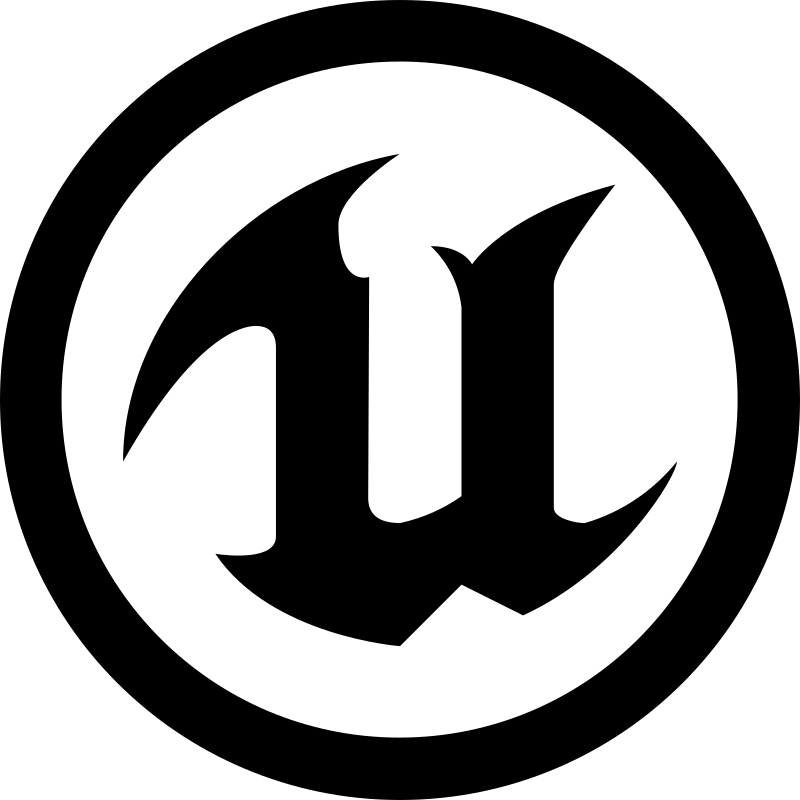
\includegraphics[width=0.2\textwidth]{./Figuras/Aspectos/UnrealLogo.png}\label{fig:UnrealLogo}}
	\hfil
	\subfigure[Godot Engine.]{
\includegraphics[width=0.2\textwidth]{./Figuras/Aspectos/GodotLogo.png}\label{fig:GodotLogo}}
	\caption[Logotipos de motores Unity, Unreal Engine y Godot Engine.]{Logotipos de los motores de videojuegos mencionados en el párrafo anterior.}
	\label{fig:GameEngineLogos}
\end{figure}

Hemos seleccionado Unity para nuestro caso específico por diversas razones, dado que la aplicación se desarrolla completamente en 2D y nuestra plataforma objetivo son los dispositivos móviles, en particular las tabletas. Unity domina el 50\% del desarrollo de videojuegos para móviles, consolas y PC, con un 71\% de los 1000 mejores juegos móviles creados en Unity (\cite{PLARIUM:2024}).

El motor gráfico 2D de Unity ofrece diversas herramientas útiles para el desarrollo, como el Sprite Editor. Además, Unity tiene una sólida integración de físicas 2D que permite simular colisiones, gravedad y otros elementos físicos. Su interfaz es intuitiva y fácil de usar, como se muestra en la \autoref{fig:UnityUI}, facilitando la creación rápida de videojuegos.

\begin{figure}[h!]
	\centering
	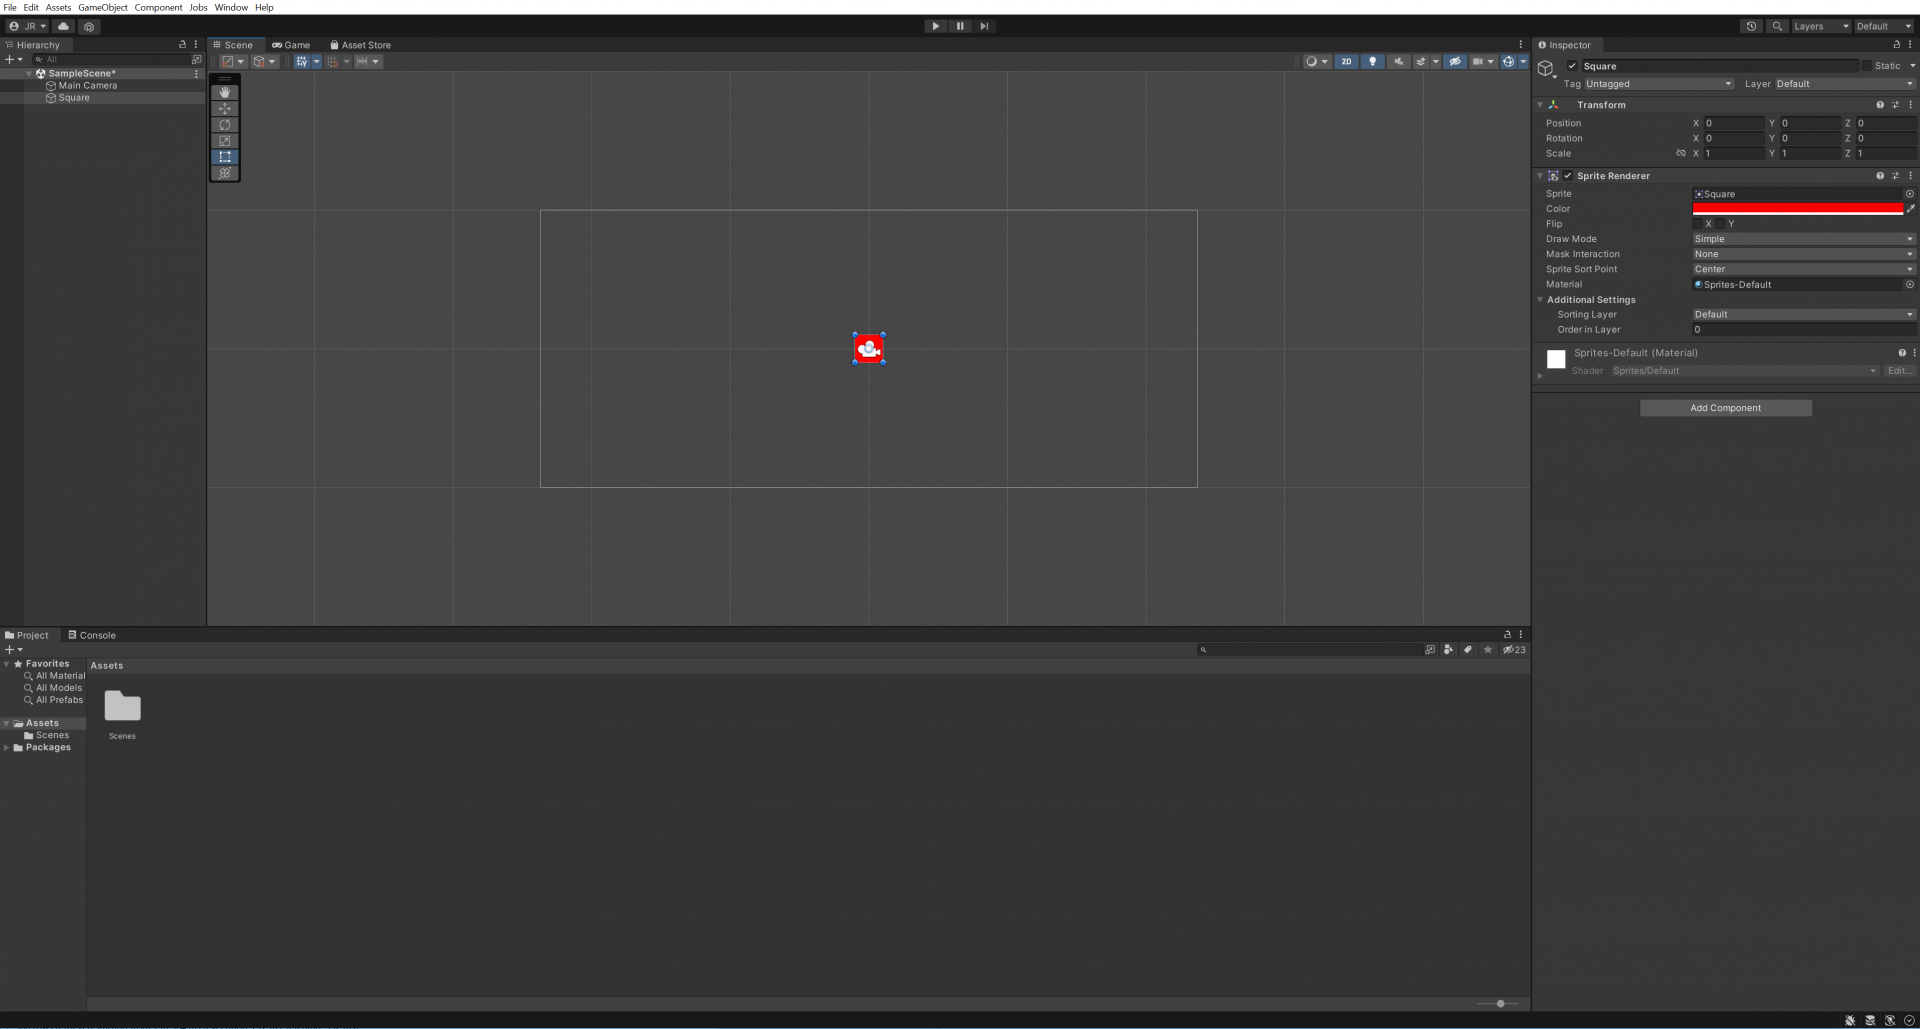
\includegraphics[width=0.8\linewidth]{./Figuras/Aspectos/UnityUI.png}
	\caption{Interfaz de usuario de la plantilla 2D de Unity.}
	\label{fig:UnityUI}
\end{figure}

La capacidad de arrastrar y soltar objetos en el editor de Unity simplifica significativamente el proceso de diseño, permitiendo a los desarrolladores centrarse en la creatividad y la jugabilidad en lugar de en aspectos técnicos complejos. Además, Unity cuenta con una comunidad amplia y activa que ofrece acceso a foros, tutoriales, cursos en línea y documentación extensa. Esta comunidad es un recurso invaluable para obtener soporte y encontrar soluciones a problemas comunes, aprender técnicas nuevas y compartir experiencias.

La Asset Store de Unity ofrece una gama variada de recursos como sprites, animaciones, scripts y plugins, que pueden agilizar el desarrollo. Estos recursos preconstruidos permiten a los desarrolladores integrar rápidamente elementos visuales y funcionales complejos sin la necesidad de crearlos desde cero, ahorrando tiempo y esfuerzo.

Todos estos factores, sumados a que Unity es el motor en el que más experiencia tenemos, fueron decisivos para seleccionarlo como el motor de desarrollo para ARTEMIS. La versión seleccionada es la 2021.3.31f, que fue la última versión de soporte a largo plazo (LTS) disponible en el momento en que se inició el proyecto.

\subsection{Visual Studio 2022 (C\#)}

Visual Studio es un entorno de desarrollo integrado (IDE) y editor de código, creado por Microsoft en 1997. Este editor es compatible con numerosos lenguajes de programación, como C++, Visual Basic .NET, Fortran, J\# y, más relevante para nuestro desarrollo, C\#. Su versión 2022 es la última versión disponible actualmente, y ha incorporado mejoras de rendimiento y nuevas funciones de accesibilidad para el usuario. Visual Studio, junto con Visual Studio Code y JetBrains Rider, forma el conjunto de editores de código con la mejor integración con Unity.

\subsection{FMOD}

FMOD Studio es un middleware\footnote{Un middleware, en términos de informática, es un software que facilita la comunicación entre las distintas aplicaciones y el sistema operativo. Además, proporciona funcionalidades inteligentes que permiten una innovación más rápida y un desarrollo eficiente. En el desarrollo de videojuegos, el middleware es un software que facilita la implementación de funcionalidades específicas dentro del motor.} de audio para videojuegos. Fue desarrollado y lanzado por Fireflight Technologies en 1995. Este motor de música y efectos de sonido se asemeja a un DAW tradicional, como se puede observar en la \autoref{fig:FMODUI}. FMOD Studio pertenece a la misma familia que el middleware Audiokinetic Wwise. Ambos proveen herramientas para la sonorización de videojuegos que facilitan la implementación de audio. Sin embargo, se ha decidido utilizar FMOD Studio debido a la mayor familiaridad con este software.

\begin{figure}[h!]
	\centering
	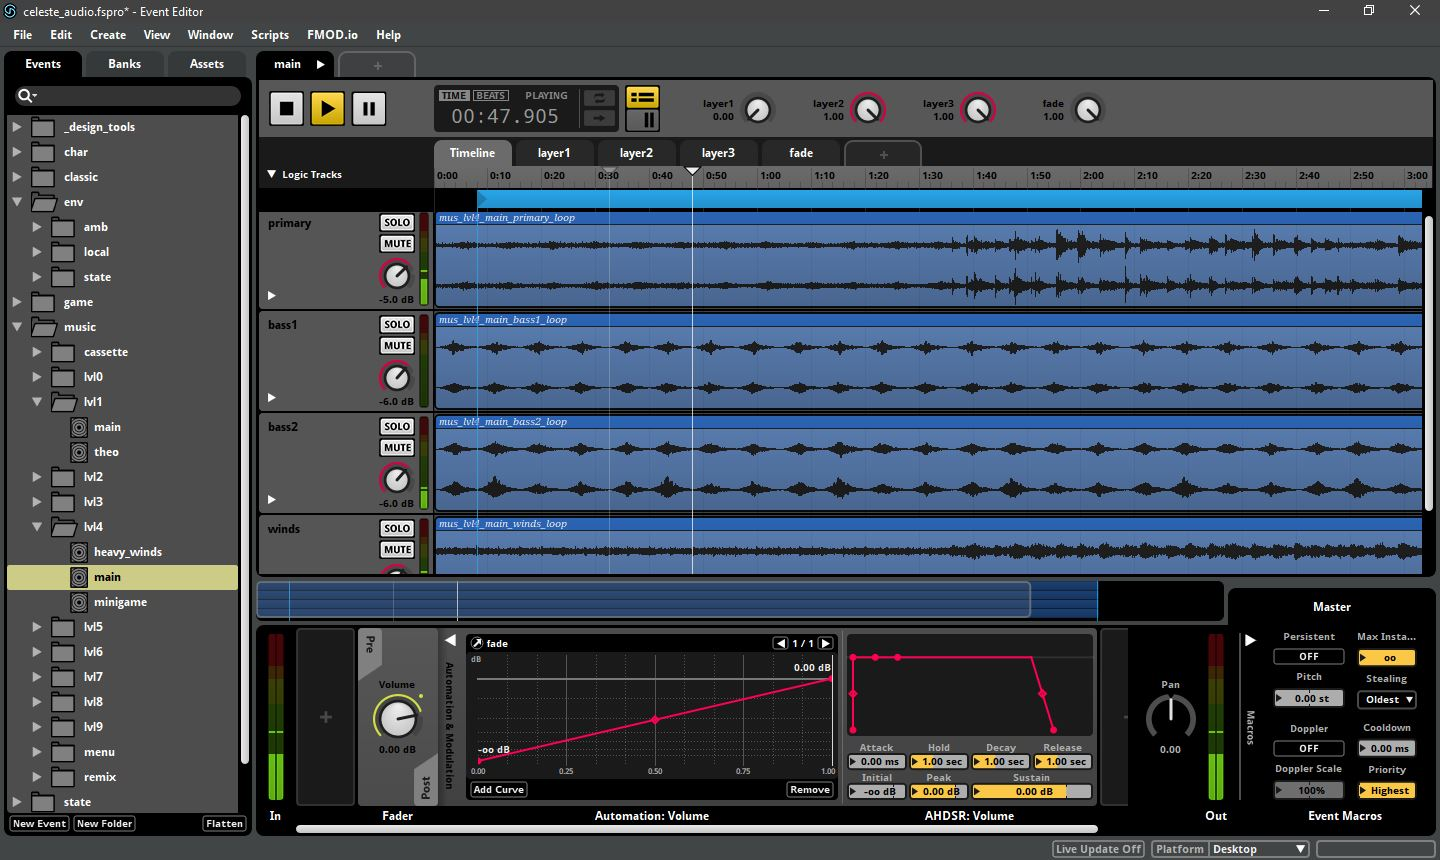
\includegraphics[width=0.9\linewidth]{./Figuras/Aspectos/FMODStudio.jpg}
	\caption[Interfaz de usuario de FMOD Studio.]{Interfaz de usuario de FMOD Studio. \\ \textbf{Fuente:} 
	}
	\label{fig:FMODUI}
\end{figure}

A diferencia del sistema de audio de Unity, que tiene funcionalidades limitadas, FMOD Studio permite gestionar con gran precisión las pistas de audio en eventos, incluso utilizando filtros de diversos tipos si fuera necesario. Desde FMOD Studio, se pueden añadir parámetros asociados a zonas de bucle, compases musicales o pistas, que luego pueden ser modificados desde los propios componentes de Unity o por programación de scripts en función de las necesidades del videojuego que se esté desarrollando.

\subsection{TeXstudio}

TeXstudio es un editor de LaTeX de código abierto lanzado en 2009 que ofrece un soporte moderno para la escritura. Cuenta con funcionalidades como la corrección ortográfica interactiva, el plegado de código y el resaltado de sintaxis. La decisión de utilizar un editor de LaTeX en lugar de editores de texto convencionales, como Word, se basa en la magnitud del documento. LaTeX ofrece citación y referencia automáticas de figuras o tablas, proporcionando estabilidad y sostenibilidad al documento. También permite almacenar toda la bibliografía en una base de datos con toda la información relevante de la cita, incluyendo referencias sobre el autor, fecha, enlaces y otros datos de interés. Los datos se pueden citar manualmente o automáticamente según un sistema de citas específico, en nuestro caso APA 7. Al combinarse con la distribución Miktex, la instalación automática de paquetes y la actualización a las últimas versiones tanto de los paquetes como de TeXstudio, asegura mantener siempre actualizado el software.

\subsection{GitHub}

GitHub es un repositorio que utiliza el control de versiones de Git para alojar proyectos. La utilización de GitHub ha facilitado la colaboración entre los distintos miembros del grupo de investigación, permitiendo a cada uno trabajar en diferentes aspectos del proyecto de forma simultánea. Tiene un sistema de revisión de código, en forma de pull requests\footnote{Un pull request es una solicitud en la que un colaborador solicita al administrador que revise los cambios que ha realizado, antes de fusionarlos con la rama principal del proyecto.}, que asegura que todos los cambios tengan que ser aprobados antes de poder ser integrados en la rama principal del proyecto, añadiendo una capa de protección que otorga seguridad al código. Tiene integración directa con Unity y LaTeX, por lo que ha sido muy útil para permitir el trabajo remoto entre los distintos miembros del grupo de investigación e incluso para trabajar en distintos dispositivos sin necesidad de migrar manualmente el proyecto. El uso del repositorio nos ha brindado una serie de comodidades que, sin su utilización, habrían obstaculizado el progreso eficiente del proyecto, ya sea por las posibles restricciones geográficas del equipo o por el número de miembros que lo conforman.

% CAPÍTULO 4 - DESARROLLO DEL TRABAJO
\chapter{Desarrollo del trabajo}  
%\addcontentsline{toc}{chapter}{\numberline{}Desarrollo del trabajo}
El proyecto de investigación ARTEMIS es una iniciativa interdisciplinaria que reúne el trabajo de varios estudiantes de diferentes especialidades y campos. Este enfoque colaborativo permite abordar el proyecto desde diversas perspectivas, enriqueciendo así el desarrollo y la implementación de soluciones innovadoras. ARTEMIS se centra en el diseño y desarrollo de aplicaciones digitales interactivas. Estas han sido específicamente desarrolladas para realizar terapias de estimulación emocional a través del arte y la música, utilizando la tecnología como vehículo principal. Además, estas aplicaciones están diseñadas para ser intuitivas y accesibles, permitiendo a los usuarios interactuar con ellas de manera sencilla. Este proyecto tiene como objetivo integrar las últimas innovaciones tecnológicas con prácticas terapéuticas tradicionales, para potenciar los beneficios emocionales y psicológicos de los pacientes. A pesar de que cada uno de los estudiantes que conforman el equipo se ha centrado en líneas de investigación particulares, todos comparten objetivos comunes que han guiado sus esfuerzos hacia una meta colectiva.

Para contribuir al conocimiento científico y hacer funcionales las terapias diseñadas, las aplicaciones permiten la configuración por edades y patologías. Se definen pruebas psicométricas\footnote{Los test psicométricos son largos ya que consisten en alrededor de 30-40 preguntas. Al final de cada aplicación o sesión, se realizan preguntas rápidas del tipo termómetro.} al inicio y al final de la actividad, y los datos recogidos\footnote{La definición del perfil del paciente implica una entrevista entre el terapeuta y el paciente, donde se indaga acerca de su historia musical, gustos y características relacionadas con la música. El terapeuta será el encargado de introducir una serie de datos en la aplicación para optimizar esta fase.} de los pacientes se almacenan para su posterior consulta por el terapeuta. Los datos recogidos incluyen la edad, el nivel escolar, si se ha estudiado algún instrumento y el instrumento preferido del paciente. El perfil del paciente determina la complejidad musical en, por ejemplo, la composición interactiva. Un perfil con menos experiencia musical tendrá la capacidad de entender una complejidad musical menor o menos disonante, mientras que un perfil con más experiencia puede manejar una armonía más elaborada. Es importante mencionar que estas aplicaciones tienen una función de doble usuario en la que tanto el terapeuta como el paciente participan simultáneamente, cada uno con un rol específico. El terapeuta actúa como instructor, guiando al paciente en su interacción con la aplicación. 

La primera fase del proyecto ARTEMIS se ha enfocado en el tratamiento de la ansiedad infantil, utilizando la tecnología como vehículo para la transición emocional, complementándose con terapias tradicionales basadas en musicoterapia. La estructura de las sesiones terapéuticas es modular y se puede adaptar a las necesidades individuales del paciente. Cada sesión comienza con la definición del perfil del paciente y luego se selecciona una o más actividades vinculadas directamente a las líneas de investigación previamente definidas, en las que profundizaremos más en detalle en los próximos párrafos. Dentro de cada actividad, se han desarrollado una o más aplicaciones con distintos enfoques, que pueden ser utilizadas en función de las observaciones del terapeuta. Las actividades que han servido como punto de partida para el desarrollo de estas aplicaciones, y que han dado lugar a las líneas de investigación, son:

\begin{itemize}
	\item \textbf{Actividad 1 - Psicoeducación emocional:} esta primera actividad se enfoca en entender la emoción, específicamente la ansiedad, y en cómo combatirla. El educador, que en este caso es el terapeuta, proporciona de manera concisa información científica relevante para responder a preguntas importantes. El paciente recibe una serie de herramientas que le ayudan a identificar, comprender y manejar la ansiedad.
	\item \textbf{Actividad 2 - Relajación guiada mediante la respiración:} el terapeuta, con la ayuda del soporte digital, guía al paciente a realizar ejercicios de relajación centrados en la respiración. El paciente sincroniza sus respiraciones con la interacción tecnológica, aportando un elemento artístico que acompaña la respiración.
	\item \textbf{Actividad 3 - Ordenar pensamientos a través del ritmo:} el paciente se centra en utilizar el ritmo como herramienta para organizar sus pensamientos y emociones. Bajo la guía del terapeuta, se establece un escenario rítmico que permite al paciente explorar y organizar sus ideas y sentimientos de una manera ordenada, respetando siempre su subjetividad.
	\item \textbf{Actividad 4 - Improvisación:} se basa en la completa libertad del paciente, donde, a través de la improvisación musical, el paciente debe expresar su estado de ánimo.
	\item \textbf{Actividad 5 - Repetición de patrones rítmicos:} el paciente debe escuchar y repetir patrones rítmicos con la mayor precisión posible con el objetivo de controlar la impulsividad. 
\end{itemize}

Estas actividades constituyen la base sobre la que se han construido para las distintas aplicaciones, respaldadas por las líneas de investigación. Estas líneas se han establecido para abordar los objetivos del proyecto desde una perspectiva multidisciplinaria, uniendo las cuatro áreas de estudio: arte, tecnología, música y terapias de estimulación emocional. Las líneas de investigación son las siguientes:

\begin{itemize}
	\item Musicoterapia y narrativa audiovisual.
	\item Musicoterapia y arte digital.
	\item Musicoterapia y composición interactiva.
	\item Musicoterapia y diseño de videojuegos (serious games).
	\item UX/UI interacción y branding.
\end{itemize}

Abordaremos cada línea de investigación individualmente, indagando en profundidad en sus aplicaciones derivadas. Específicamente, la aplicación más relevante para este TFG se encuentra en la línea de investigación de diseño de videojuegos con musicoterapia. Dejaremos esta para el final con el fin de explicarla en mayor detalle, ya que es él núcleo principal de este trabajo.

\section{Musicoterapia y narrativa audiovisual}

La narrativa audiovisual es una parte integral del proyecto de investigación. Está presente en todas las aplicaciones, en mayor o menor medida, y actúa como un vínculo entre todas ellas. El objetivo de contar una historia es proporcionar información al paciente de manera que pueda sentirse identificado y conectar directamente con sus emociones. Dado que estamos estudiando la ansiedad, es importante explicar al paciente cómo funciona e involucrarlo en la explicación integrada en forma de historia. Hemos definido tres elementos en la narrativa que están directamente relacionados con este enfoque, y cuyo objetivo es involucrar activamente al paciente.

\begin{itemize}
	\item \textbf{Personaje principal:} es el elemento más crítico de la narrativa. Su función es actuar como un espejo que permite al paciente identificarse, y sirve como guía para el mismo. Este personaje es una especie de Pepito Grillo\footnote{Pepito Grillo es un personaje de ficción creado para Las Aventuras de Pinocho (\cite{LADP:1883}), que Walt Disney Pictures, actual Walt Disney Studios, adaptó en 1940 en la película de animación Pinocho. En la cultura popular, Pepito Grillo representa una figura de confianza a quien recurrimos para obtener consejo. Esta figura nos ayuda a identificar nuestros errores y no teme cuestionarnos cuando nos equivocamos.}, cuyo objetivo es ayudar al paciente a comprender su problema y a encontrar una solución.
	\item \textbf{Nivel de explicación:} dependiendo de la edad a la que se dirige la narrativa, el nivel de profundidad debe variar y adaptarse\footnote{Por ejemplo, los niños pequeños suelen utilizar el pensamiento mágico, como un duende malo que nos pone nerviosos, mientras que los adolescentes necesitan ejemplos más concretos y realistas.}. El objetivo es lograr que el paciente se identifique con el ejemplo situacional que la historia propone. Para que esto suceda, es esencial usar analogías para explicar las leyes del mundo.
	\item \textbf{Píldoras mínimas:} para que la historia sirva como un nexo cohesivo entre las aplicaciones, debe quedar claro cuál es el objetivo de la actividad específica que se va a realizar. Debe responder a la pregunta: ¿Cuál es la finalidad de lo que estoy a punto de hacer?
\end{itemize}

Todos estos elementos se centran en lo que se conoce como inmersión contextual. Esto implica el estudio del contexto de los pacientes para introducir elementos que se ajusten a las circunstancias de cada uno. El objetivo es promover una identificación adecuada entre el paciente, su situación y la historia.

La historia principal debe unir todas las actividades de forma natural sin perder el objetivo que acabamos de comentar. Esta historia, escrita por Isabel Xiaowei de San Sebastián para ARTEMIS, se puede resumir de la siguiente manera:

\begin{adjustwidth}{100pt}{0pt}
	\noindent "\textit{El protagonista es un ser del bosque que nació de una flor, gracias al poder de una ninfa. La diosa Artemis ha perdido su magia y el protagonista ayuda a recuperarla. Su misión es buscar semillas de diente de león perdidas en el bosque para entregárselas a la ninfa, quien las transforma en flores. En su travesía, se encuentra con varios desafíos, representados por actividades terapéuticas, que debe completar para avanzar. El nivel no concluye hasta que se completan todas las actividades. Una vez finalizado un nivel, el protagonista puede repetirlo o continuar con la historia. Las ninfas, en intervalos regulares, se reúnen con las distintas flores de cada emoción que han creado a partir de las semillas y se las entregan a Artemis. Cada emoción se representa como una planta distinta, personalizando así la estética del personaje con diferentes plantas. Existe una escala del dolor que, dependiendo del nivel de ansiedad del paciente, muestra diferentes elementos que ayuden al terapeuta a comprender la situación del paciente.}"
\end{adjustwidth}

La ambientación de esta historia está fuertemente vinculada con la naturaleza, que se asocia con la relajación y vitalidad. Así, los elementos estéticos deben ser coherentes con este tema. Considerando que ARTEMIS se centra en la ansiedad infantil, los elementos estéticos se diseñan para adecuarse a este contexto. Esta estética, repleta de colores vivos y personajes con rasgos de la animación tradicional, busca establecer una conexión con su público objetivo. Como no podemos determinar el género del paciente que utilizará la aplicación, decidimos desde el principio que el personaje debía ser andrógino. En la \autoref{fig:MainCharacterConcept}, observamos que se intentó alcanzar este objetivo desde las primeras propuestas estéticas. La versión final del personaje mantiene la androginia, combinando rasgos humanos con elementos naturales. Se puede comparar la versión inicial con la final en la \autoref{fig:MainCharacter}.

\begin{center}
	\textbf{Fuente:} Realizado por Sergio Calvo, miembro ARTEMIS.
	\vspace{-18pt}
\end{center}

\begin{figure}[h!]
	\centering
	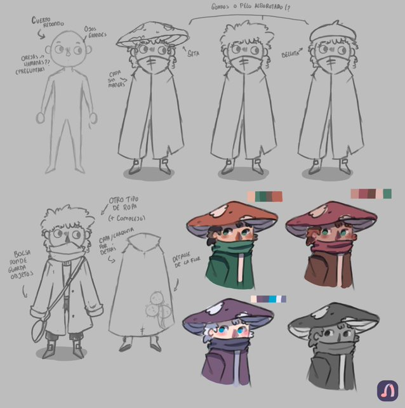
\includegraphics[width=0.4\linewidth]{Figuras/Desarrollo/PersonajesNuevosConcept}
	\caption{Propuesta inicial de personaje principal.}
	\label{fig:MainCharacterConcept}
\end{figure}

\begin{center}
	\textbf{Fuente:} Realizado por Isabel Xiaowei de San Sebastián, miembro ARTEMIS.
	\vspace{-18pt}
\end{center}

\begin{figure}[h!]
	\centering
	\subfigure[Primera iteración del personaje.]{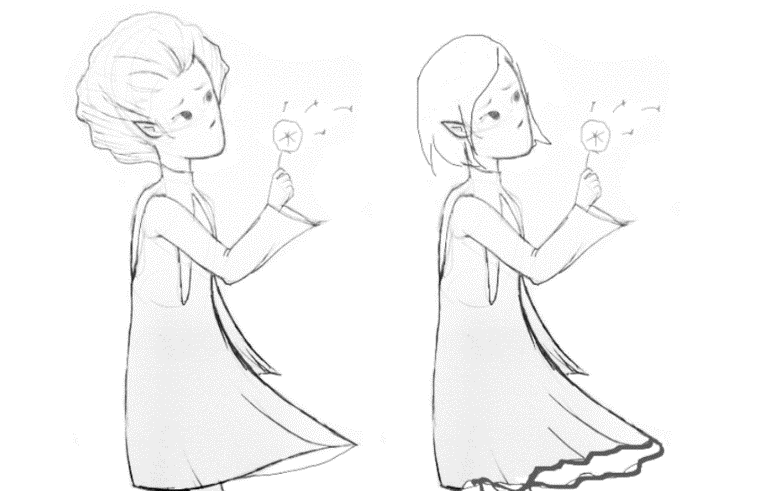
\includegraphics[width=0.4\textwidth]{./Figuras/Desarrollo/PersonajesAntiguos.png}\label{fig:MainCharacterOld}}
	\hfil
	\subfigure[Última iteración del personaje.]{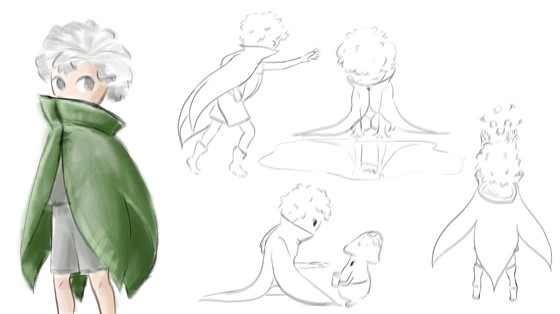
\includegraphics[width=0.4\textwidth]{./Figuras/Desarrollo/PersonajesNuevos.jpg}\label{fig:MainCharacterNew}}
	\caption{Evolución de la conceptualización del personaje principal.}
	\label{fig:MainCharacter}
\end{figure}

Las ninfas, musas y gracias tienen una fuerte relación con la música y pueden ser los personajes identificados con instrumentos que el protagonista encuentra en su aventura. Por esta razón, los personajes secundarios que el protagonista encuentra a lo largo de la narrativa portan instrumentos (como se puede observar en la \ref{fig:InstrumentCharacters}), representando físicamente a estos seres.

\begin{center}
	\textbf{Fuente:} Realizado por Isabel Xiaowei de San Sebastián, miembro ARTEMIS.
	\vspace{-18pt}
\end{center}

\begin{figure}[h!]
	\centering
	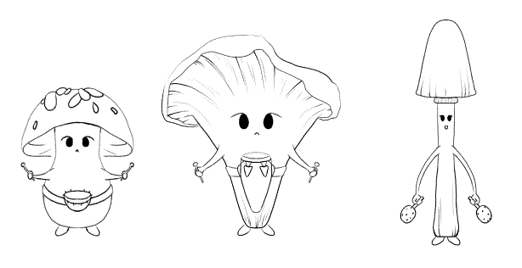
\includegraphics[width=0.3\linewidth]{Figuras/Desarrollo/InstrumentCharacters}
	\caption{Propuesta de concepto de personajes con instrumentos.}
	\label{fig:InstrumentCharacters}
\end{figure}

Antes de concluir esta línea de investigación, es relevante describir el formato que fundamenta esta historia y cómo se lleva a cabo la interacción del paciente bajo la guía del terapeuta. La historia se visualiza a través de un libro ilustrado interactivo. De este modo, el terapeuta puede controlar el ritmo de la historia y, si es necesario, retroceder. Para avanzar, se debe pulsar manualmente el botón de pasar página, permitiendo al terapeuta determinar cuánto tiempo se necesita en cada página, en caso de tener que explicar algún detalle.
La ansiedad tiende a inquietar a quien la padece. Por ello, un sistema que permite adaptar el ritmo de la narrativa a cada situación, permite al terapeuta elegir el enfoque más beneficioso para el paciente en cuestión.

\begin{center}
	\textbf{Fuente:} \citeauthor{LORIRI:2018} (\citeyear{LORIRI:2018}).
	\vspace{-18pt}
\end{center}

\begin{figure}[h!]
	\centering
	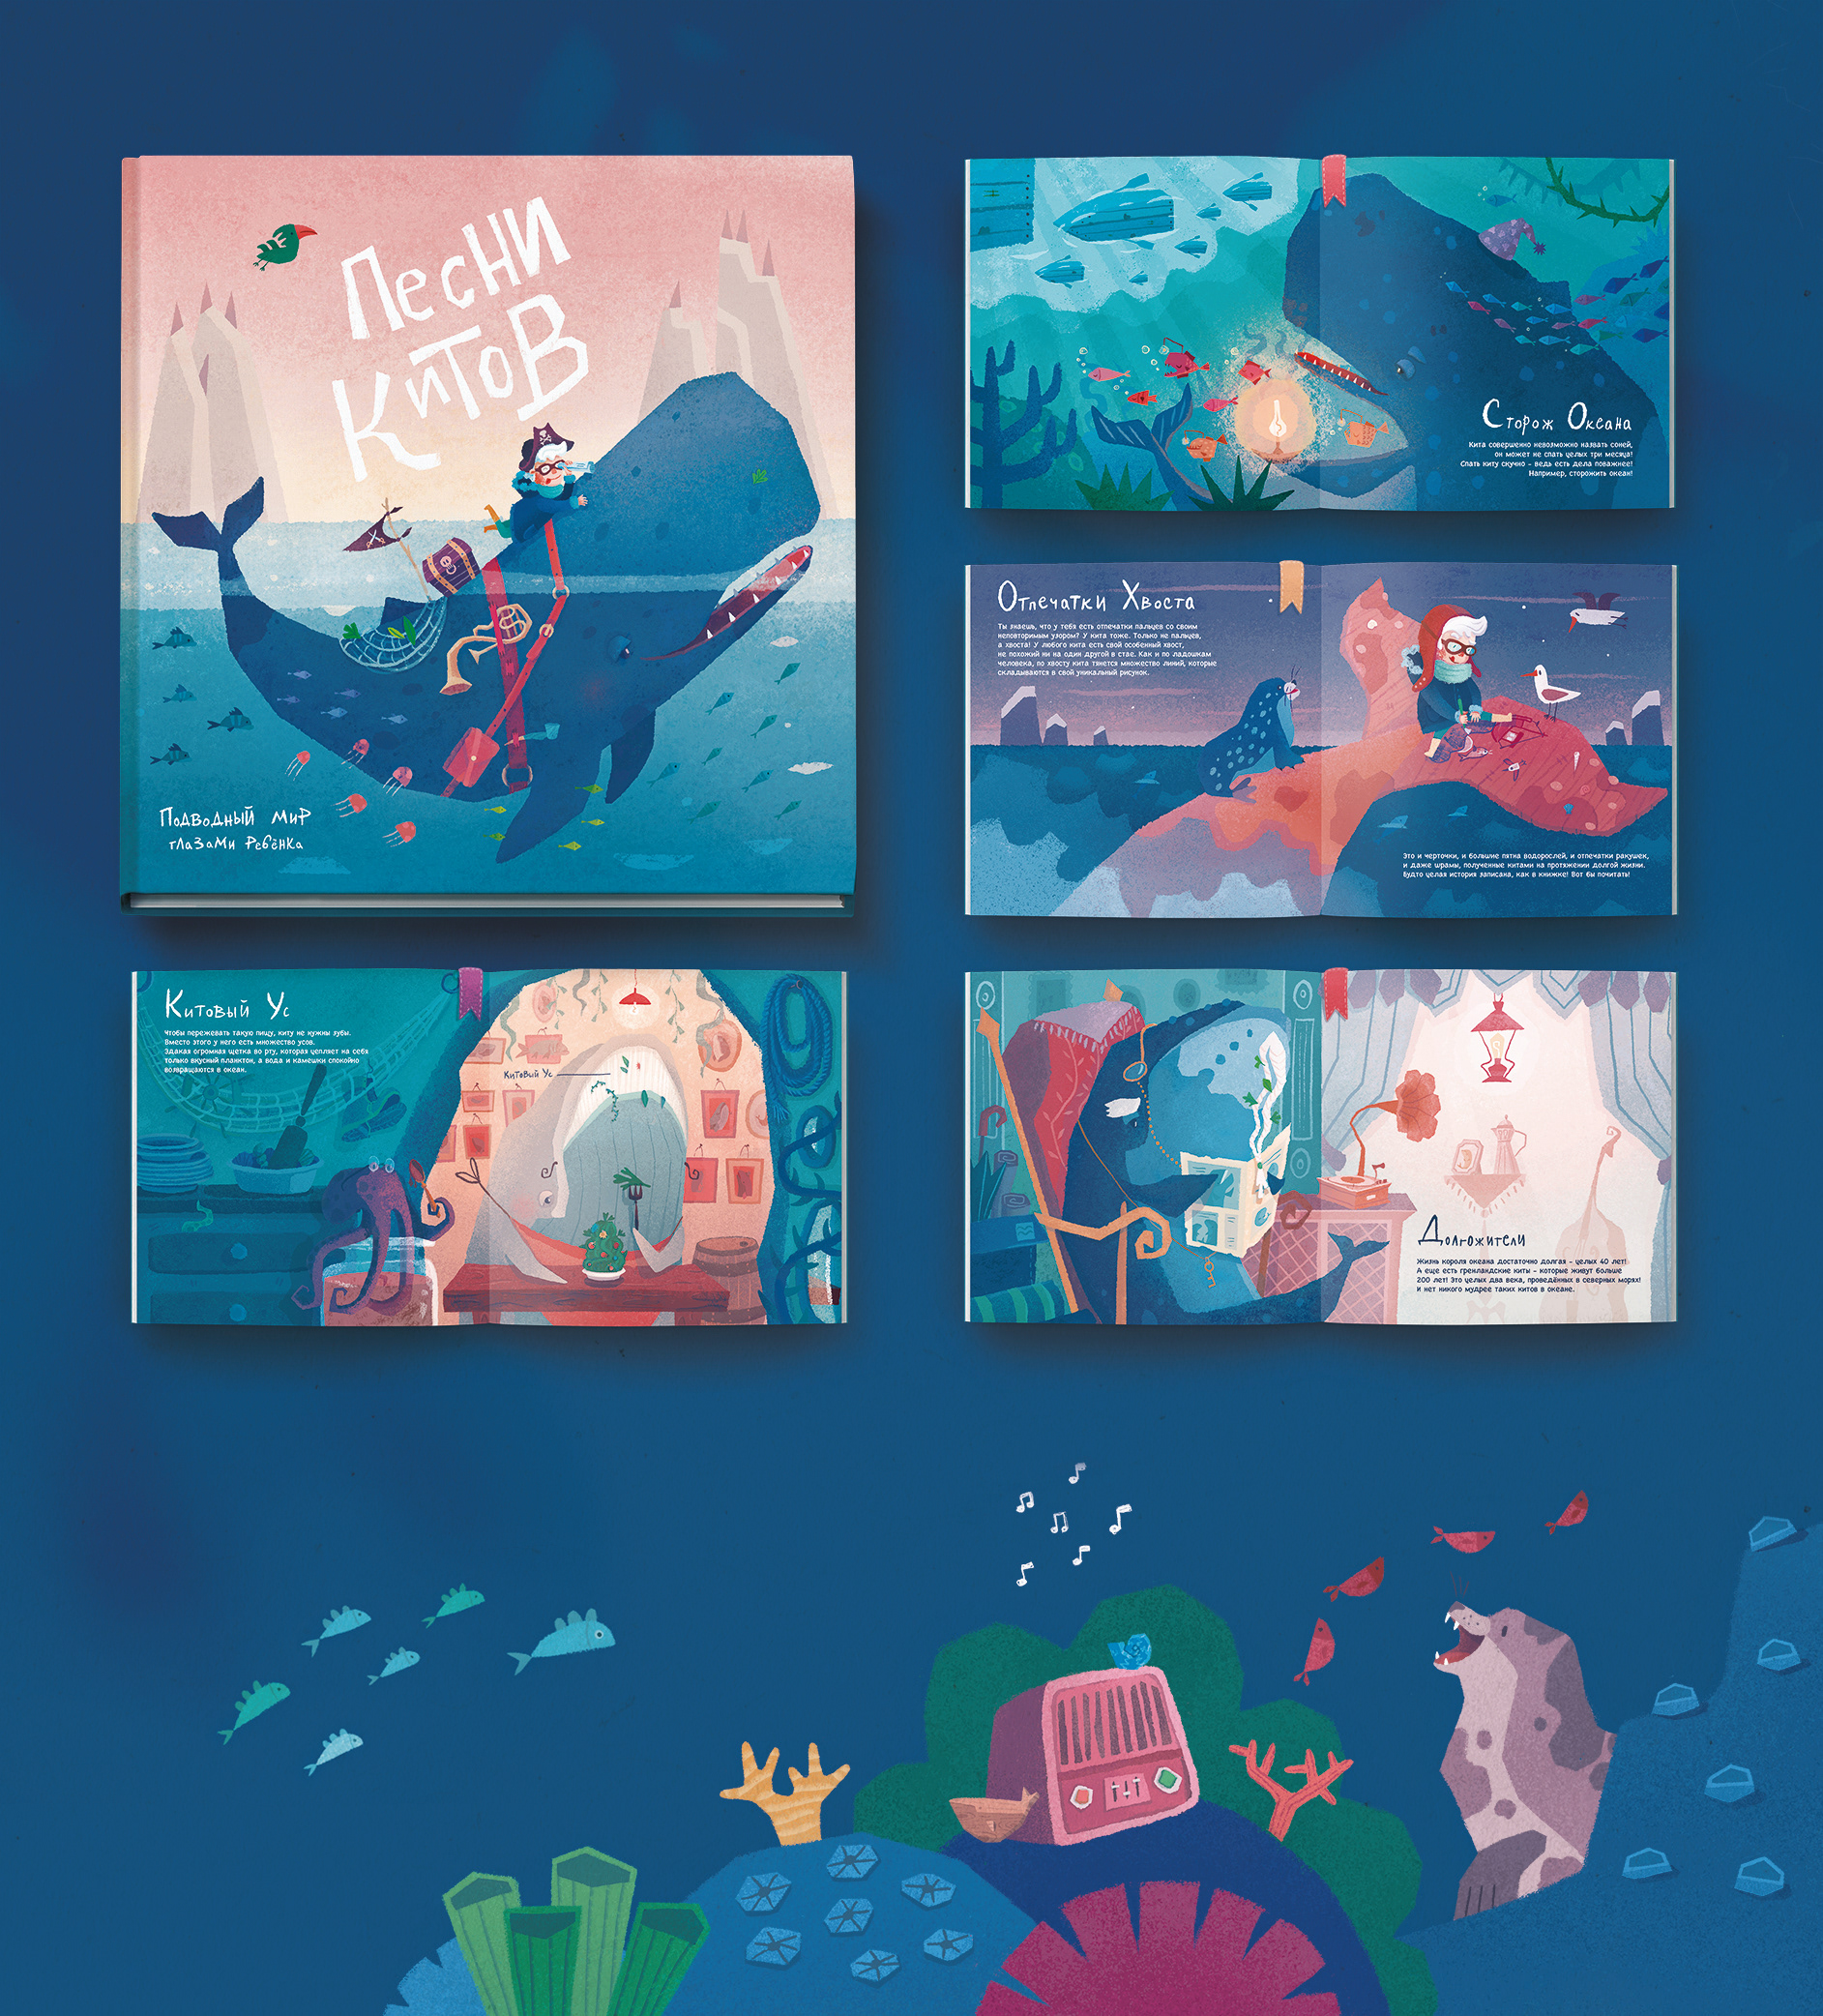
\includegraphics[width=0.4\linewidth]{Figuras/Desarrollo/ImagenReferenciaLibro.jpg}
	\caption{Imagen de referencia de libro interactivo.}
	\label{fig:LoriRiBook}
\end{figure}

\begin{center}
	\textbf{Fuente:} Realizado por Isabel Xiaowei de San Sebastián, miembro ARTEMIS.
	\vspace{-18pt}
\end{center}

\begin{figure}[h!]
	\centering
	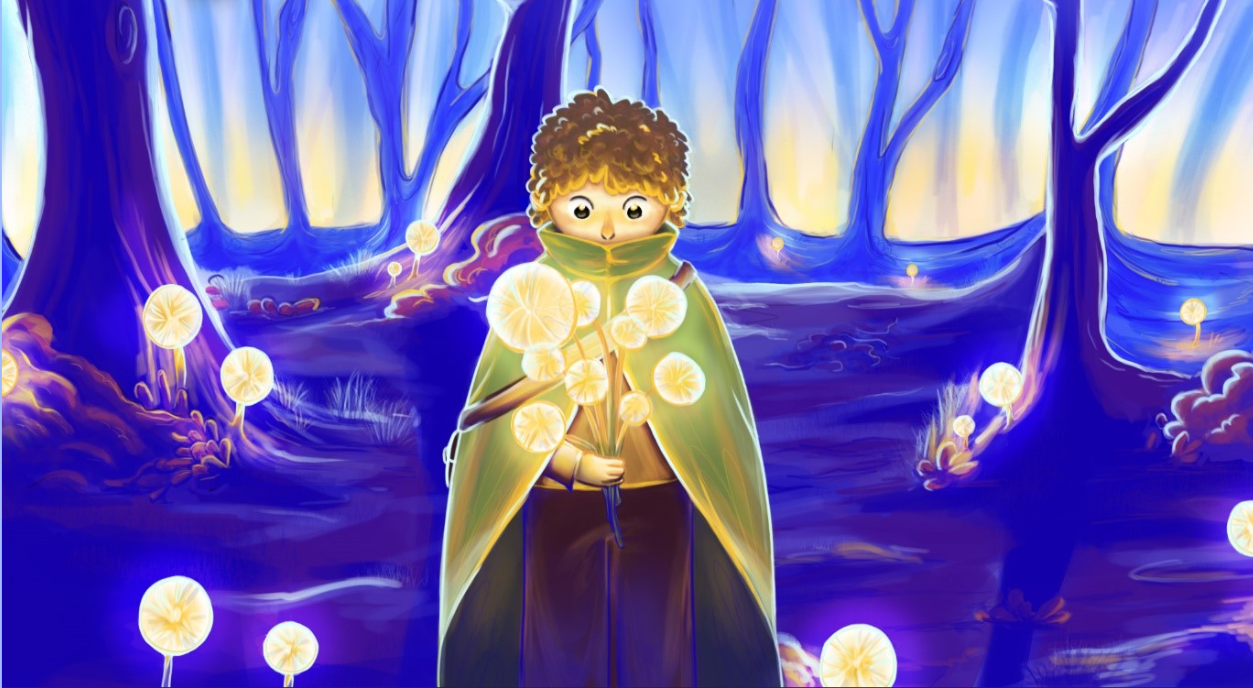
\includegraphics[width=0.5\linewidth]{Figuras/Desarrollo/IlustracionLibro.png}
	\caption{Ilustración de ejemplo del libro ilustrado interactivo.}
	\label{fig:BookIllustration}
\end{figure}

La narrativa es un elemento fundamental para la identificación del paciente con la aplicación. Esta aumenta la eficacia de la terapia en función del grado de inmersión que la tecnología pueda proporcionar en las sesiones de musicoterapia.

\section{Musicoterapia y arte digital}

La línea de investigación en arte digital propone una pieza de arte digital interactiva. Esta pieza, mediante experiencias visuales y música, puede ayudar en la gestión emocional y facilitar la transición de una emoción a otra a través de la interacción del usuario. Los datos de interacción se pueden recoger a través de la información proporcionada por periféricos comunes como una tableta y sus sensores (cámara o pantalla táctil). El objetivo de este recurso es ayudar al paciente a concentrarse y relajarse, enseñándole cómo respirar visualmente en situaciones de ansiedad. La interacción con esta herramienta se realiza mediante pulsaciones táctiles, ya sean cortas o prolongadas, o movimientos de la mano frente a la cámara. Se espera que estas acciones sean guiadas por el terapeuta para alcanzar su objetivo. De esta manera, al no usar un micrófono que puede generar varios problemas dependiendo del tipo de paciente que recibe la terapia\footnote{Usar un micrófono como sistema principal de entrada puede causar problemas en ciertos casos aislados. Las voces más graves producen ondas de sonido que son más difíciles de capturar, por lo que no sería correcto limitar las terapias a personas con voces más reconocibles.}, se evitan complicaciones. En términos de salida de la experiencia, la parte visual se mostrará en la pantalla y la parte musical se emitirá a través de altavoces o auriculares. Las propuestas de visualización para esta pieza se pueden dividir en dos categorías: visual y musical.

\begin{itemize}
	\item \textbf{Apartado visual:} se genera un mar de partículas que oculta un paisaje, siguiendo la línea estética del proyecto. Este paisaje se revela mediante la animación de las partículas, las cuales se ven afectadas por el contacto del dedo del paciente al deslizarse por la pantalla. Este movimiento depende de la longitud de la exhalación.
	\item \textbf{Apartado musical:} se reproduce una melodía relajante de fondo con sonidos que nos recuerdan a la naturaleza (el viento, la vegetación, los animales, etc). Por otro lado, al interactuar con la pieza, también se emite un sonido más fuerte de brisa, que emula la exhalación.
\end{itemize}

\begin{center}
	\textbf{Fuente:} \citeauthor{VAMOSS:2023} (\citeyear{VAMOSS:2023}).
	\vspace{-18pt}
\end{center}

\begin{figure}[h!]
	\centering
	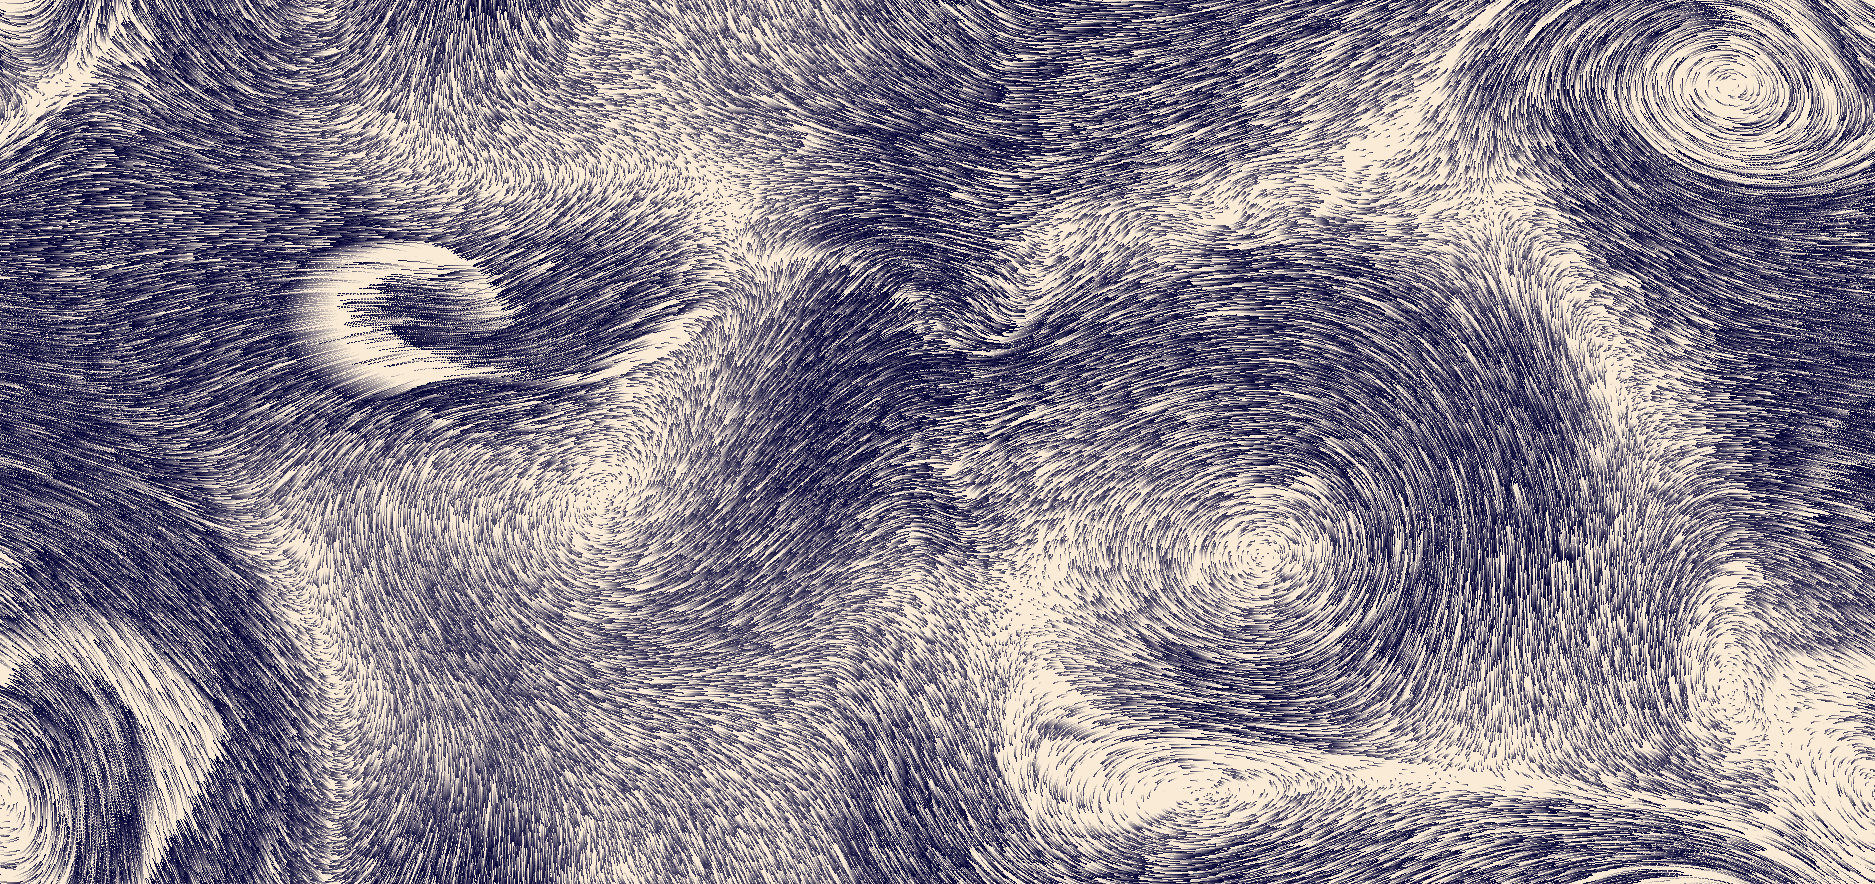
\includegraphics[width=0.4\linewidth]{Figuras/Desarrollo/MarParticulas.png}
	\caption{Referencia principal de arte interactivo en relación con la propuesta de Clara Guoshi, miembro de ARTEMIS. En el enlace de la referencia bibliográfica, se puede probar la experiencia creada por Vamoss.}
	\label{fig:SeaParticles}
\end{figure}

\section{Musicoterapia y composición interactiva}

La composición interactiva se basa en la creación de música como una forma de expresión libre. Mediante la modificación en tiempo real de un tema musical o combinaciones musicales, se pueden generar variaciones melódicas y paisajes sonoros. A través de esta interacción, el paciente puede crear música sencilla. Esta línea de investigación presenta dos aplicaciones. Aunque son diferentes, ambas buscan utilizar los mismos métodos para alcanzar el objetivo.

\subsection{Aplicación 1: Paisaje sonoro}

El paisaje sonoro, que se inspira en referencias como Reactable\footnote{Reactable es un instrumento musical electrónico colaborativo desarrollado por el Grupo de Tecnología Musical de la Universidad Pompeu Fabra en Barcelona. Este instrumento permite a los usuarios crear topologías musicales complejas y dinámicas mediante la colocación y rotación de elementos físicos en su interfaz. Está inspirado en los sintetizadores modulares de los años sesenta y permite el uso de generadores, filtros y moduladores para la creación musical.} o Incredibox (\citeauthor{INCREDIBOX:2023}, \citeyear{INCREDIBOX:2023}), se centra en la creación de música a través de la selección de los instrumentos que participarán en la melodía. Esta aplicación tiene como objetivo acomodar a aquellos pacientes con menor conocimiento musical, reforzando la simplicidad requerida para que estas aplicaciones sean utilizadas por su público objetivo. En realidad, no existe una solución incorrecta, lo que permite al paciente sentir que tiene el control de la música y evitar la frustración de no poder crear una melodía armoniosa.

La aplicación consta de cuatro niveles distintos, cada uno asociado a un género musical. Esto permite al terapeuta seleccionar los instrumentos con los que desea trabajar, en función de las necesidades del paciente. Además, la aplicación puede utilizarse de manera indefinida, hasta que el paciente o el terapeuta decidan finalizar su uso. La idea principal de la aplicación es que los instrumentos generan un paisaje musical, asociando cada elemento con aspectos de la naturaleza, como flores o árboles. Este paisaje cambia según el género musical seleccionado. Los cuatro géneros que agrupan los distintos instrumentos, junto con algunos ejemplos de instrumentos, son:

\begin{itemize}
	\item \textbf{Música clásica:} piano, violín, viola, trompeta, trombón, percusión, violonchelo, oboe, corno, fagot, clarinete, contrabajo, flauta traversa o flauta de pico.
	\item \textbf{Música pop-rock:} voz, guitarra eléctrica, bajo, batería, teclados, guitarra acústica, sintetizador o caja de ritmos.
	\item \textbf{Música caribeña o latina:} gaitas, arco musical, caña de millo, guacharaca, guache, tablitas, bombos, redoblantes, platillos, campanas o tambor.
	\item \textbf{Música electrónica:} sintetizador, caja de ritmos, theremin o sonidos generados por ordenador.
\end{itemize}

Cada uno de estos géneros representa un paisaje específico, aludiendo a las cuatro estaciones. Los elementos de fondo y la paleta de colores cambian, pero siempre se mantiene el aspecto natural.La aplicación, desarrollada por Ángela García, miembro de ARTEMIS, incluye un menú inicial donde se puede seleccionar el género deseado y la pantalla de juego, donde se puede observar en acción lo que hemos mencionado anteriormente. En la \autoref{fig:SonoricEnvironment}, se pueden observar ambas interfaces.

\begin{center}
	\textbf{Fuente:} Realizado por Ángela García, miembro ARTEMIS.
	\vspace{-18pt}
\end{center}

\begin{figure}[h!]
	\centering
	\subfigure{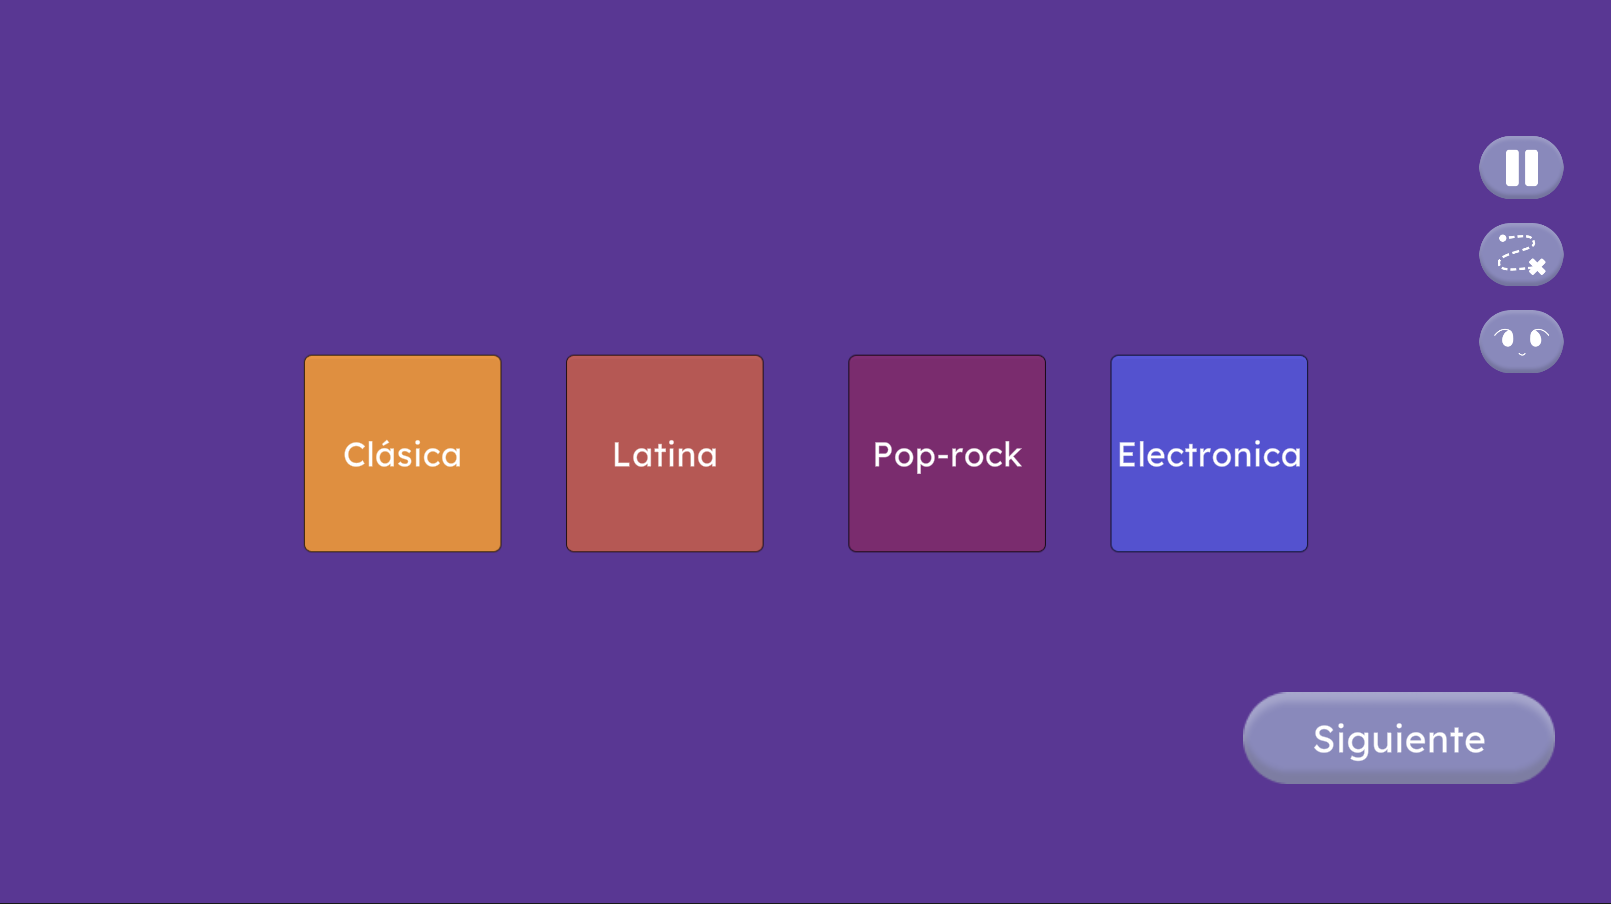
\includegraphics[width=0.4\textwidth]{./Figuras/Desarrollo/PaisajeSonoroMenu.png}\label{fig:SonoricEnvironmentMenu}}
	\hfil
	\subfigure{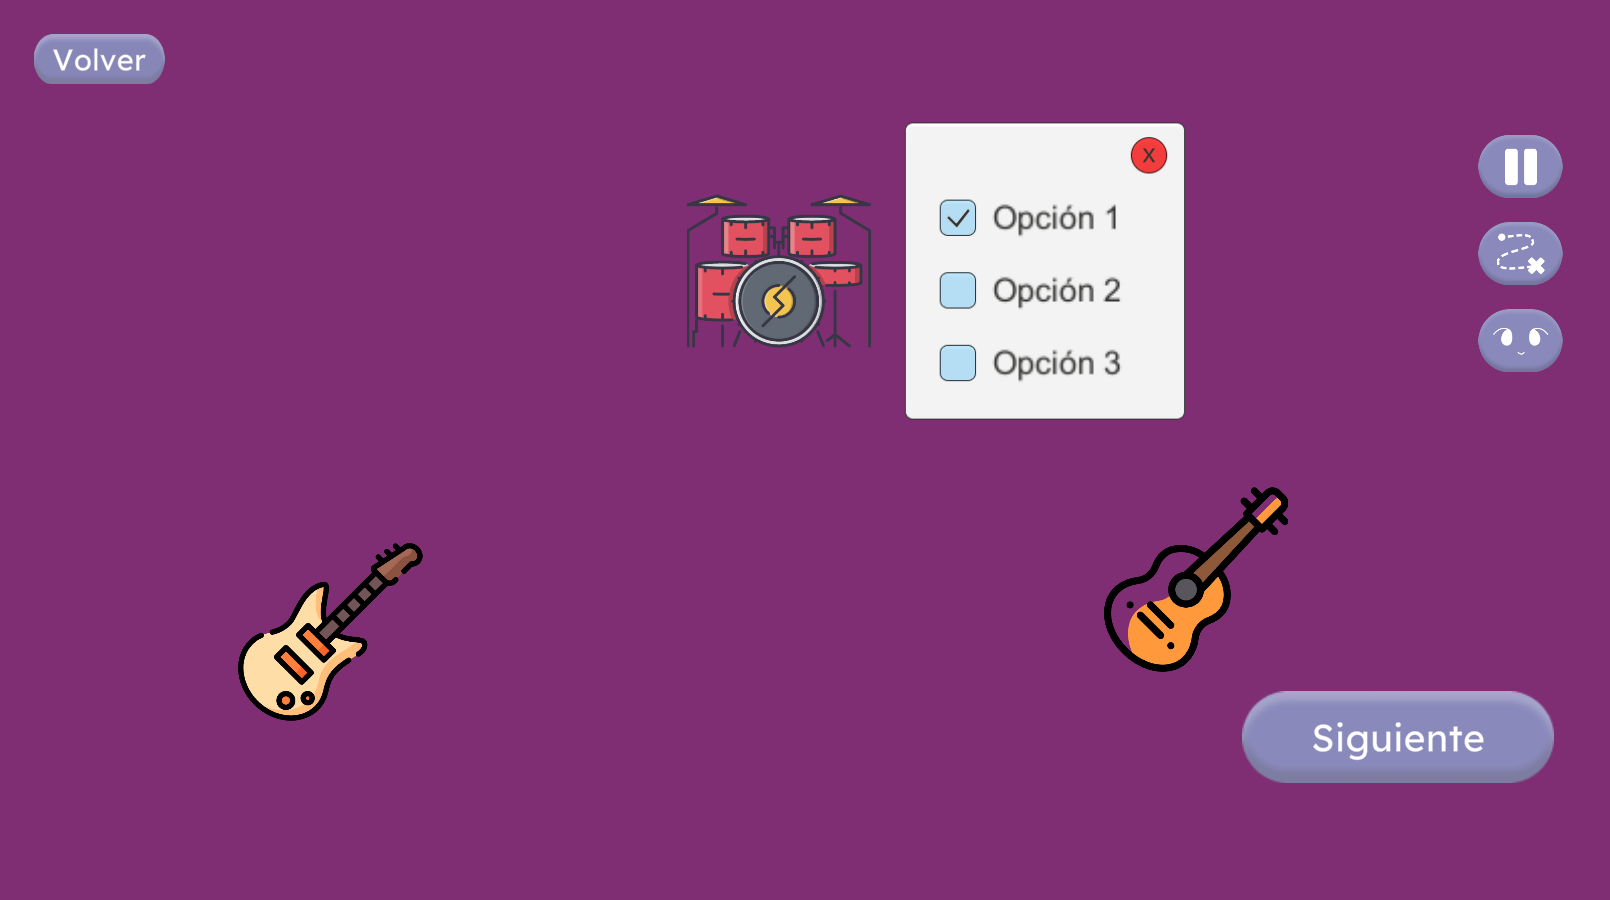
\includegraphics[width=0.4\textwidth]{./Figuras/Desarrollo/PaisajeSonoroGame.png}\label{fig:SonoricEnvironmentGame}}
	\caption{Pantallas del menú y del juego en la aplicación de paisaje sonoro.}
	\label{fig:SonoricEnvironment}
\end{figure}

\begin{center}
	\textbf{Fuente:} Realizado por Leticia Gómez, compositora ARTEMIS.
	\vspace{-14pt}
\end{center}

\begin{figure}[h!]
	\centering
	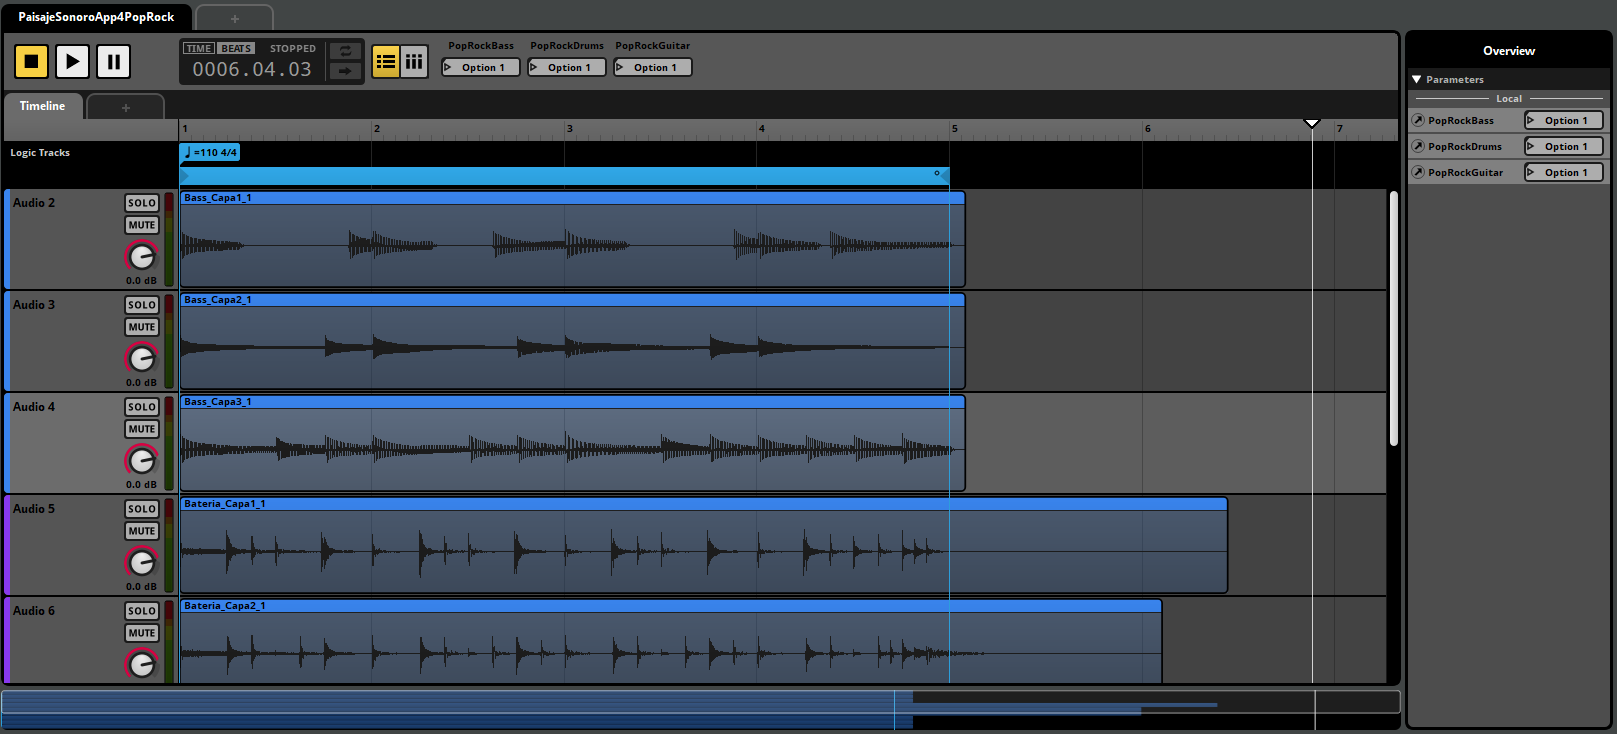
\includegraphics[width=0.8\linewidth]{Figuras/Desarrollo/PaisajeSonoroFMOD.png}
	\caption[Interfaz de FMOD aplicación paisaje sonoro.]{Interfaz de FMOD con los contenidos del género pop-rock de la aplicación de paisaje sonoro.}
	\label{fig:SonoricEnvironmentFMOD}
\end{figure}

A nivel musical, la aplicación utiliza FMOD para sincronizar rítmicamente las diversas pistas de audio y los parámetros para alternar entre ellas. Se puede observar en la \autoref{fig:SonoricEnvironmentFMOD}, cómo está configurado el middleware de audio para garantizar el correcto funcionamiento de la aplicación. Cada evento de FMOD engloba un género específico. Aquí se agrupan todas las pistas de audio por instrumentos, que se reproducen según los parámetros indicados a través de scripting dentro de Unity.

\subsection{Aplicación 2: Melodía floral}

A diferencia de la aplicación anterior, esta tiene una complejidad musical mayor, requiriendo un entendimiento teórico previo para su uso. Sin embargo, los conceptos utilizados en la aplicación son bastante sencillos para que un niño sin experiencia musical pueda aprenderlos rápidamente, tras una breve explicación del terapeuta. Al mismo tiempo, son lo suficientemente profundos para que un niño con experiencia musical pueda desenvolverse cómodamente con sus conocimientos adquiridos previamente. La aplicación de melodía floral incluye un pentagrama interactivo que permite cambiar tanto la duración como la altura de las notas. Por ello, es necesario conocer la nomenclatura musical, aunque no necesariamente de las notas, pero sí de los tipos de duración que existen, como las redondas, blancas, negras, corcheas, o incluso, los silencios.

\begin{center}
	\textbf{Fuente:} Realizado por Isabel Xiaowei de San Sebastián, miembro ARTEMIS.
	\vspace{-18pt}
\end{center}

\begin{figure}[h!]
	\centering
	\subfigure{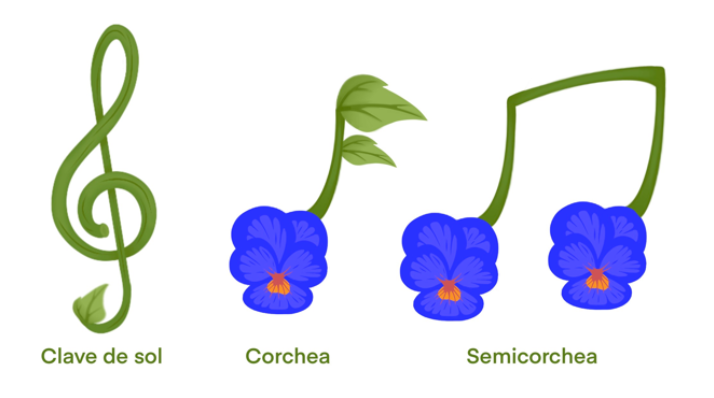
\includegraphics[width=0.45\textwidth]{./Figuras/Desarrollo/MelodiaFloralNotas1.png}\label{fig:FloralMelodyNotes1}}
	\subfigure{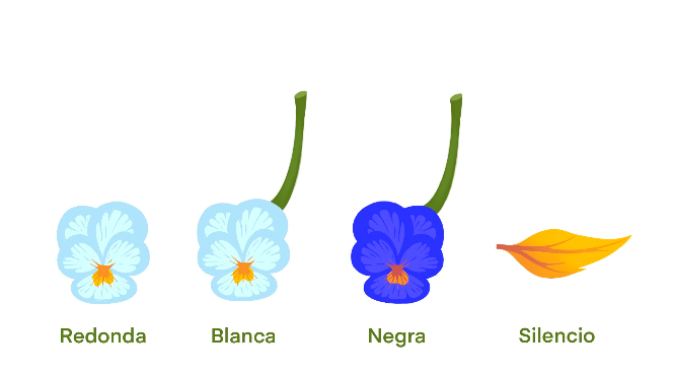
\includegraphics[width=0.45\textwidth]{./Figuras/Desarrollo/MelodiaFloralNotas2.png}\label{fig:FloralMelodyNotes2}}
	\caption{Representación visual de las figuras musicales en función de su duración.}
	\label{fig:FloralMelodyNotes}
\end{figure}

En cada iteración de la aplicación, se carga una melodía de una biblioteca, que el terapeuta puede seleccionar según las necesidades del paciente. Una vez seleccionada, aparece un pentagrama clásico con las notas dispuestas de acuerdo con la melodía. La estética de la aplicación conserva un aspecto natural, y cada nota se representa con un tipo de flor. La flor cambiará dependiendo de la duración de la nota, con las notas negras representadas por flores más oscuras y las notas blancas por flores literalmente blancas. Los silencios se representan con una hoja otoñal caída. Una gran referencia para la aplicación es el editor de melodías de Animal Crossing: New Horizons (\cite{ACNH:2020}), que permite la creación musical a través de la colocación de notas y silencios, variando la altura de las mismas. 

Este enfoque visual ofrece varios beneficios terapéuticos. La representación visual de las notas como flores y hojas ayuda a los pacientes a conectarse emocionalmente con la música, haciendo que la experiencia sea más significativa. Además, la visualización de las notas y silencios facilita la comprensión de la teoría musical, incluso para aquellos sin conocimientos previos. La capacidad de crear y modificar melodías permite a los pacientes expresarse de manera creativa, lo cual puede ser especialmente útil para la liberación emocional y la exploración de sentimientos.

\begin{center}
	\textbf{Fuente:} Realizado por Elisa Alonso, miembro ARTEMIS.
	\vspace{-18pt}
\end{center}

\begin{figure}[h!]
	\centering
	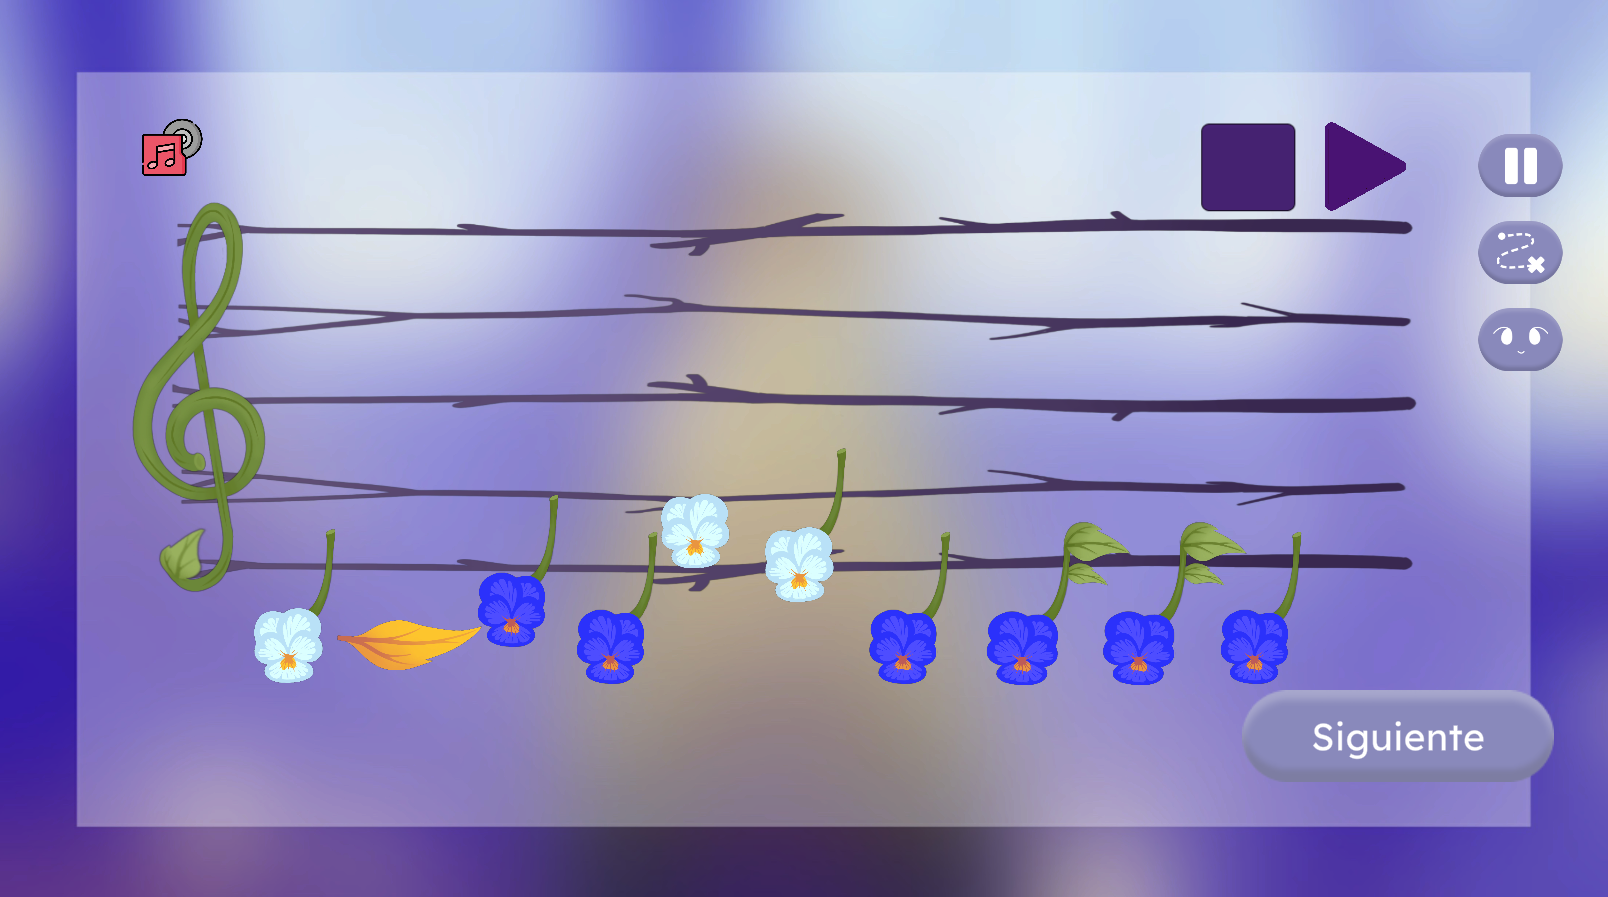
\includegraphics[width=0.8\linewidth]{Figuras/Desarrollo/MelodiaFloralGame.png}
	\caption[Interfaz de la aplicación melodía floral.]{Interfaz de la aplicación de melodía floral, mostrando un ejemplo de notas a distintas alturas y con diferentes figuras.}
	\label{fig:FloralMelodyGame}
\end{figure}

En la \autoref{fig:FloralMelodyGame}, se muestra un ejemplo visual de una secuencia de notas con sus respectivas representaciones de duración. Cuando el usuario presiona el botón de inicio (triángulo equilátero horizontal), las notas se reproducirán una a una con las alturas correspondientes y la duración especificada. También es posible modificar las notas mientras la secuencia está en ejecución, lo que permite escuchar los cambios en tiempo real.

Ambas aplicaciones, con el objetivo de permitir que el paciente exprese sus sentimientos, utilizan una serie de elementos únicos que determinan la profundidad del diseño y los casos de uso. Estos elementos permiten al terapeuta adaptar la aplicación y darle al paciente la libertad de expresar cómo se siente. Además, estas aplicaciones no solo están diseñadas para terapias individuales, sino que también ofrecen posibilidades para terapias grupales, facilitando la colaboración y socialización a través de ciertas dinámicas de grupo. En el contexto grupal, estas aplicaciones permiten a los pacientes trabajar juntos en la creación de melodías y compartir sus experiencias emocionales, fortaleciendo así las relaciones interpersonales entre ellos y el terapeuta.

La composición interactiva busca crear un entorno seguro donde los pacientes pueden explorar libremente sus sentimientos, fomentando la autoexpresión. La musicoterapia se complementa significativamente con la composición interactiva digital, aprovechando la capacidad expresiva de la música en entornos digitales. Estos entornos permiten el uso de visuales emocionantes junto con sistemas modulares adaptables a diversas situaciones. En función de la creación musical del paciente y la información que este proporcione al terapeuta, se puede obtener información valiosa para adaptar con mayor facilidad las sesiones terapéuticas.

\section{Musicoterapia y diseño de videojuegos (serious games)}

El diseño de videojuegos y la musicoterapia pueden parecer campos distintos inicialmente, pero tienen varios puntos en común que los vuelven complementarios en un contexto terapéutico. Los videojuegos, diseñados para ser interactivos, mantienen la atención del usuario, siempre que el diseño sea adecuado. Esta interactividad puede ser aplicada en la musicoterapia para involucrar activamente a los pacientes en su terapia. La posibilidad de interactuar con el entorno digital hace la terapia más dinámica y atractiva para el paciente. Además, la gamificación de las terapias mejora la participación de los pacientes. Sin duda, el mayor desafío en la gamificación de terapias es lograr un equilibrio; el juego debe ser interesante pero sin llegar a frustrar al paciente. El objetivo de incorporar el diseño de videojuegos en las terapias de musicoterapia es motivar a los pacientes a participar activamente, con el fin de alcanzar sus objetivos terapéuticos.

Los videojuegos son conocidos por utilizar una combinación de elementos visuales y auditivos para crear experiencias inmersivas, combinadas con la interacción, que es lo que lo diferencia de otros formatos audiovisuales como el cine. En la musicoterapia, estos elementos pueden ser utilizados para fortalecer la conexión emocional del paciente con la música. La creación de estas experiencias interactivas sumergen al paciente en un entorno enriquecido que facilita la expresión emocional. Es importante enfatizar que la motivación que deben tener los pacientes debe ser intrínseca. No debe estar ligada a ninguna recompensa más allá del propio placer de disfrutar jugando. La herramienta tecnológica tiene como objetivo ser un complemento, y que el simple hecho de utilizarla pueda ayudar al paciente sin necesidad de recompensas adicionales. La verdadera recompensa radica en el tránsito emocional, de emociones con connotaciones negativas a emociones con connotaciones positivas. Estas aplicaciones funcionan como un doble usuario donde terapeuta y paciente interactúan para alcanzar los objetivos de la terapia. El videojuego actúa como un núcleo de cooperación entre ambas partes, guiados por el terapeuta, para obtener mejores resultados. Además, el diseño de terapias grupales fomenta la interacción social y el apoyo mutuo entre los pacientes. 

Esta línea de investigación, compuesta por dos aplicaciones, se basa en el diseño de videojuegos para crear experiencias interactivas que sean atractivas para el paciente y útiles para el terapeuta en su labor por dirigir la terapia. La primera aplicación, llamada Harmony Heaven, utiliza el concepto de la exploración como un puzle. La segunda aplicación, Ritmo Vegetal, presenta un puzle que consiste en resolver una situación aparentemente caótica, pero sin existir una solución incorrecta, ya que esta será subjetiva para el paciente. Nos centraremos en detallar la primera aplicación y dejaremos la segunda para más adelante en el documento. Esto se debe a que la segunda aplicación es la más relevante para este TFG, ya que constituye la base de todo el trabajo del autor en el proyecto ARTEMIS.

\subsection{Aplicación 1: Harmony Heaven}



Está sección es la más relevante de este RFG ya que conforma todo el trabajo del autor sobre el proyecto ARTEMIS.




% CAPÍTULO 5 - CONCLUSIONES
\chapter{Conclusiones}  
%\addcontentsline{toc}{chapter}{\numberline{}Conclusiones}
\section{Conclusión}

La ansiedad es una emoción común en la vida humana, presente desde la niñez hasta la vejez. Es probable que tengamos que lidiar con sus síntomas en algún momento de nuestras vidas. El proyecto ARTEMIS se creó para proporcionar soporte digital a las terapias psicológicas enfocadas en el tratamiento de las emociones con connotaciones negativas mediante la musicoterapia. Para esta etapa del proyecto en concreto, la investigación se centró alrededor del tratamiento de la ansiedad. Al inicio de este TFG, se fijaron unos objetivos generales y específicos que se alinearon con los del proyecto ARTEMIS. El objetivo principal se ha centrado en desarrollar una aplicación con enfoque de videojuego serio, basándose en los principios del proyecto. Los objetivos secundarios, en cambio, han incluido el estudio de estructuras musicales para identificar patrones que los pacientes puedan integrar en sus creaciones musicales, así como el análisis del impacto de las experiencias interactivas digitales en las prácticas tradicionales de musicoterapia.

A lo largo del trabajo se han cumplido los distintos objetivos en sus respectivas secciones. Tanto el estudio de las estructuras musicales como el análisis del impacto de las experiencias interactivas digitales en musicoterapia se han realizado en el marco teórico. Con el conocimiento de las figuras rítmicas y el proceso de composición, se pueden crear piezas musicales que relajen al paciente. Además, si la pieza es creada por el propio paciente, la satisfacción en su creación es subjetiva, facilitando el proceso de mejora. Las experiencias interactivas digitales no solo aumentan la interacción entre el terapeuta y el paciente, sino que también sitúan a ambos en una situación de doble usuario donde pueden cooperar para alcanzar el objetivo principal de la terapia. Es importante destacar que la adaptabilidad de este formato permite al terapeuta ajustar las terapias fácilmente según las necesidades del paciente. Lograr cumplir ambos objetivos desemboca en el desarrollo de la aplicación que no solo debe ser funcional desde un punto de vista terapéutico, sino que también debe tener la capacidad de establecer una conexión emocional entre el terapeuta y el paciente para facilitar una comunicación efectiva.

En rasgos generales, la investigación se enfocó en los pilares fundamentales del proyecto ARTEMIS: las emociones (específicamente la ansiedad), el ritmo y la creación musical, la musicoterapia y el desarrollo de videojuegos serios. Todos estos temas, que abarcan las áreas de conocimiento de la psicología, la música y los videojuegos, se exploraron a fondo en el marco teórico. En primer lugar, se definieron el ritmo y sus componentes principales (pulso, tempo y métrica) utilizando diversas fuentes. Citamos a \citeauthor{CASTELLANOS:2009} (\citeyear{CASTELLANOS:2009}) y su explicación de cómo el ritmo juega un papel esencial en la música, permitiendo marcar el tiempo de una pieza musical. Es similar a cómo miramos el reloj para realizar ciertas acciones. Además, el ritmo, siendo un movimiento cíclico, tiene una gran relación con la inhalación y exhalación de la respiración. Este aspecto confiere al ritmo un potencial terapéutico de grandes dimensiones.

Se exploró también el proceso de composición musical y las diversas maneras de componer música. Utilizamos el trabajo de \citeauthor{SUBIRATS:2004} (\citeyear{SUBIRATS:2004}) para investigar los diferentes niveles de creatividad que otorgan diversas habilidades en la creación. Es importante destacar la diferencia entre la improvisación libre y la composición guiada. Ambos tipos de creación son útiles en entornos terapéuticos y, combinados con las diferentes formas de generar música, brindan a los terapeutas un abanico de opciones para sus sesiones. Sin embargo, es necesario evaluar las necesidades del paciente para determinar qué tipo de creación musical se debe utilizar. En relación con el oyente de música, existe un término conocido como expectativa musical que juega un papel crucial en el manejo de las emociones. \citeauthor{SENABRE:2019} (\citeyear{SENABRE:2019}) expone una serie de teorías que fundamentan la expectativa musical. Estas teorías nos ayudan a comprender qué espera un paciente de su creación musical y cómo podemos ayudarle a alcanzar un resultado satisfactorio.

Para comprender la situación de un paciente con síntomas de ansiedad, fue necesario definir esta emoción, los tipos de trastornos que existen y sus tratamientos. Aunque nuestro caso de estudio está enfocado en las terapias psicológicas para tratar la ansiedad, también ampliamos la información para incluir tratamientos farmacológicos con el mismo objetivo. Se examinó la relación entre esta emoción y la musicoterapia. Antes de hacerlo, definimos qué es la musicoterapia. Nos basamos en \citeauthor{WFMT:2024} (\citeyear{WFMT:2024}), una federación especializada en musicoterapia, para comprender el verdadero significado de las terapias basadas en música. Observamos que la musicoterapia se divide en dos modalidades: activa y receptiva. En la musicoterapia activa, el paciente se encuentra en un contexto donde él es el creador de la música, mientras que en la musicoterapia receptiva, el paciente escucha música grabada o interpretada en vivo por el terapeuta. La elección entre una u otra modalidad recae en el terapeuta, quien debe evaluar las circunstancias del paciente para tomar tal decisión. Se ha demostrado que la música es un componente poderoso en el tratamiento de la ansiedad. Un estudio realizado por \citeauthor{SEPULVEDA:2014} (\citeyear{SEPULVEDA:2014}) mostró que la musicoterapia reducía drásticamente los niveles de ansiedad en pacientes infantiles con cáncer.

Finalmente, se exploraron los elementos de diseño que definen al videojuego serio, enfatizando las características que lo distinguen del formato tradicional del videojuego. Se especificó en los diferentes campos de aplicación de los videojuegos serios, como la educación o la salud, proporcionando ejemplos de desarrollos específicos cuyo objetivo era otorgar una mejora a los usuarios en cada campo particular. La investigación culminó con una recopilación de videojuegos serios para la salud, detallando sus objetivos, los elementos de diseño que incluyen y cómo podrían ser útiles en nuestro desarrollo. \textit{Operation Quest} (\cite{OPERATIONQUEST:2024}), por su enfoque hacia el público infantil; \textit{SPARX} (\cite{SPARX:2013}), por su narrativa que explica al paciente su situación; \textit{Flow} (\cite{FLOW:2006}), por su simplicidad mecánica; y \textit{Deep VR} (\cite{DEEP:2021}), por su ambiente inmersivo e innovadoras aplicaciones de interacción, proporcionan una perspectiva amplia de los objetivos del proyecto ARTEMIS.

Se decidió adoptar una metodología que imita los procesos de desarrollo de un videojuego tradicional. Las características principales en la creación de un videojuego incluyen la definición de requisitos antes de comenzar, la conceptualización y diseño de las mecánicas del juego, y el desarrollo iterativo. En nuestro caso específico, para ofrecer un diseño de juego sólido, es necesario fundamentar todas las decisiones de diseño en las investigaciones realizadas previamente. Hemos utilizado tecnologías que facilitan la creación de experiencias digitales interactivas, como Unity, la gestión de audio a través de FMOD, y el trabajo colaborativo en repositorios como GitHub. En combinación con la metodología estipulada, estas herramientas nos han permitido desarrollar una aplicación interactiva de musicoterapia, sin requerir que el equipo esté en el mismo lugar o tiempo. Aplicando esta metodología, se logró desarrollar un sistema interactivo en el que el paciente puede disfrutar de la creación musical como si resolviera un rompecabezas sonoro. La solución se encuentra en la satisfacción personal del paciente.

En conclusión, analizar el impacto de las experiencias digitales interactivas en las sesiones de musicoterapia mostró que estas no solo proporcionan un medio adaptativo que permite al terapeuta personalizar las terapias según las necesidades del paciente, sino que también sumergen al paciente en un entorno visual y sonoro artístico que puede ser más efectivo que las terapias tradicionales. Este formato permite al terapeuta tener un registro en tiempo real de la interacción del paciente con la aplicación, lo que posibilita el análisis de las necesidades del paciente al instante. Para el usuario, los efectos de la terapia son inmediatos debido a la interacción instantánea. En cuanto al desarrollo de la aplicación, que se basa en la modalidad de musicoterapia activa, se fundamenta en la investigación realizada. Combina las contribuciones de diferentes referencias para crear un puzle sonoro relajante en el que los pacientes pueden disfrutar creando música y asienta las bases de una posible ampliación futura hacia un alcance de emociones más allá de la ansiedad. La satisfacción de la resolución de este puzle reside en la búsqueda subjetiva de una solución auditiva agradable.

Este Trabajo Final de Grado no tiene pruebas empíricas que demuestren la utilización de esta aplicación en situaciones con pacientes reales; se fundamenta únicamente en las investigaciones realizadas. Aunque la intención inicial era utilizar la aplicación en terapias reales llevadas a cabo por los psicólogos asociados al proyecto ARTEMIS, la falta de tiempo impidió que esto ocurriera en esta primera etapa del proyecto. Haber podido comprobar la eficacia y recibir retroalimentación de los pacientes infantiles que sufren síntomas de algún tipo de ansiedad, nos habría permitido crear un producto final más iterado y pulido.

\section{Líneas de investigación futuras}

Aunque el proyecto ARTEMIS se ha centrado inicialmente en la ansiedad, tiene como objetivo expandir gradualmente su enfoque para tratar otras emociones a través de la musicoterapia. El desarrollo de esta aplicación establece las bases para un sistema complementario a las sesiones de terapia tradicional del terapeuta. El uso de un medio digital interactivo para el desarrollo ofrece un comportamiento modular que permite una gran escalabilidad del proyecto. Con el arte y las líneas narrativas ya definidos, la investigación de emociones adicionales solo requerirá identificar los problemas asociados con esas emociones y cómo tratarlos. El contexto artístico y narrativo ya está establecido.

%\clearpage
%\thispagestyle{empty}
%\printindex \nocite{*}
%\appendix

% REFERENCIAS
\newpage{\pagestyle{empty}}
\addcontentsline{toc}{chapter}{\numberline{}Referencias}
%https://github.com/SantiPlanet/apalike
%\bibliographystyle{apalike-es} 
%\bibliography{biblio}
\printbibliography

% ANEXO
\newpage{\pagestyle{empty}}
\markboth{Anexo}{Anexo}
\chapter*{Anexo}  
\addcontentsline{toc}{chapter}{\numberline{}Anexo}    
\section{Sistema de cuadrícula}

\subsection{Objeto cuadrícula} \label{code:grid}

\begin{lstlisting}
using System.Collections;
using System.Collections.Generic;
using UnityEngine;

public class Grid
{
	private int width;
	private int height;
	private float cellSize;
	private int[,] gridArray;
	
	public Grid(int width, int height, float cellSize)
	{
		this.width = width;
		this.height = height;
		this.cellSize = cellSize;
		
		gridArray = new int[width, height];
		
		for (int x = 0; x < gridArray.GetLength(0); x++)
		{
			for (int y = 0; y < gridArray.GetLength(1); y++)
			{
				Utils.CreateWorldText(gridArray[x, y].ToString(), null, GetWorldPosition(x, y), 20, Color.white, TextAnchor.MiddleCenter, TextAlignment.Center, 0);
			}
		}    
	}
	
	public Vector3 GetWorldPosition(int x, int y)
	{
		return new Vector3(x, y) * cellSize;
	}
}
\end{lstlisting}

\subsection{Clase ''Utils''} \label{code:gridUtils}

\begin{lstlisting}
using System.Collections;
using System.Collections.Generic;
using UnityEngine;

public static class Utils
{
	public static TextMesh CreateWorldText(string text, Transform parent, Vector3 localPosition, int fontSize, Color color, TextAnchor textAnchor, TextAlignment textAlignment, int sortingOrder)
	{
		if (color == null)
		{
			color = Color.white;
		}
		
		return CreateWorldText(parent, text, localPosition, fontSize, color, textAnchor, textAlignment, sortingOrder);
	}
	
	public static TextMesh CreateWorldText(Transform parent, string text, Vector3 localPosition, int fontSize, Color color, TextAnchor textAnchor, TextAlignment textAlignment, int sortingOrder)
	{
		GameObject gameObject = new GameObject("WorldText", typeof(TextMesh));
		Transform transform = gameObject.transform;
		transform.SetParent(parent, false);
		transform.localPosition = localPosition;
		
		TextMesh textMesh = gameObject.GetComponent<TextMesh>();
		textMesh.anchor = textAnchor;
		textMesh.alignment = textAlignment;
		textMesh.text = text;
		textMesh.fontSize = fontSize;
		textMesh.color = color;
		textMesh.GetComponent<MeshRenderer>().sortingOrder = sortingOrder;
		
		return textMesh;
	} 
}
\end{lstlisting}


\begin{lstlisting}
	using System.Collections;
	using System.Collections.Generic;
	using UnityEngine;
	
	public class GameManager : TemporalSingleton<GameManager>
	{
		[Header("Cannon")]
		[SerializeField] private Transform cannonTransform;
		[SerializeField] private float cannonForce;
		
		[SerializeField] GameObject temporalCharacter;
		
		public void Start()
		{
			ResetTransform(temporalCharacter);
		}
		
		public void ResetTransform(GameObject gameObject) {
			gameObject.transform.position = cannonTransform.position;
			gameObject.transform.rotation = cannonTransform.rotation;
			
			if (gameObject.GetComponent<Rigidbody2D>() != null) { 
				ResetGravity(gameObject.GetComponent<Rigidbody2D>());
				Launch(gameObject.GetComponent<Rigidbody2D>()); 
			}
		}
		
		private void ResetGravity(Rigidbody2D cmpRb) { cmpRb.velocity = Vector3.zero; }
		
		private void Launch(Rigidbody2D cmpRb) { cmpRb.AddForce(cannonTransform.up * cannonForce, ForceMode2D.Impulse); }
	}
\end{lstlisting}

\end{document}
